Nuestro algoritmo va chequeando en cada paso si existe alg\'un gimnasio capaz de ser vencido y, si existe, busca cual es el m\'as cercano de estos a ser vencidos, por lo tanto existir\'an casos en los cuales la soluci\'on obtenida para los mismos sea la \'optima pero para algunos no lo ser\'a.

\subsubsection*{Familias con soluci\'on obtenida igual a la \'optima}

%\begin{enumerate}
%\item No se obtiene soluci\'on por no haber las pokeparadas necesarias para ganar en todos los gimnasios.
%\item No se obtiene soluci\'on ya que la capacidad de la mochila no puede contener las pociones necesarias para vencer a un cierto gimnasio.
%\item Todos los gimnasios sin necesidad de pociones para ser vencidos.
%\item Las pokeparadas y los gimnasios se reciben en orden de la forma en la cual exista una pokeparada puntual para ir a cada gimnasio
%\end{enumerate}

\begin{center}
\textbf{Familia 1 y 2}
\end{center}

Ambas familias devolveran -1 ya que como se explico anteriomente tanto el greedy como el exacto presentan podas para estos casos sin soluci\'on por lo tanto su tiempo de ejecuci\'on tambi\'en ser\'a id\'entico.



\begin{figure} [!ht]
 \centering
  \subfloat[Familia 1: actua poda 1]{
    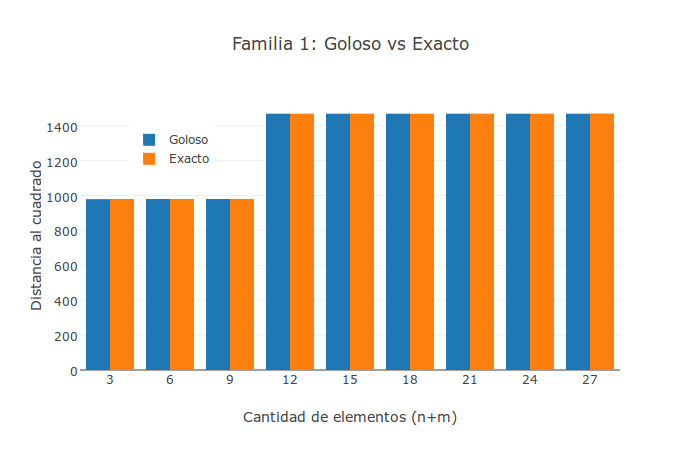
\includegraphics[width=0.45\textwidth]{./EJ2/fam1medicion.png}}
       \label{fig:jaggies}
  \subfloat[Familia 2: actua poda 2]{
    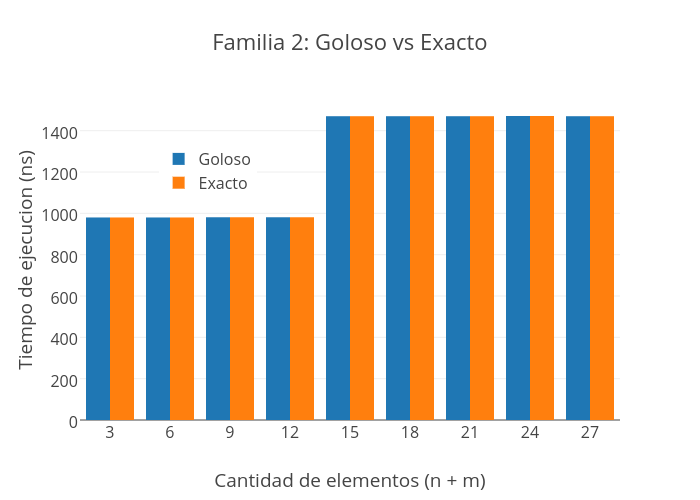
\includegraphics[width=0.45\textwidth]{./EJ2/fam2medicion.png}}
    \label{fig:moire}
    \end{figure}


Como se observa en los \'ultimos gr\'aficos, las funciones resultantes para cada familia en ambos algoritmos presentan el mismo tiempo por lo comentando sobre las podas realizadas.\\

\begin{center}
\textbf{Familia 3}
\end{center}

En este caso, como nuestro greedy chequea si hay alg\'un gimnasio a ser vencido con la cantidad de pociones que se tienen en el momento (se inicia con 0), y como todos necesitan 0, recorre los gimnasios sin necesidad de pasar por las pokeparadas, obteniendo la mejor soluci\'on posible.

A continuaci\'on mostraremos el camino obtenido tanto para el algoritmo exacto como el goloso de un caso el cual trabaja con 19 elementos en total para ejemplificar lo enunciado anteriormente:

   \vspace*{0.3cm} \vspace*{0.3cm}
  \begin{center}
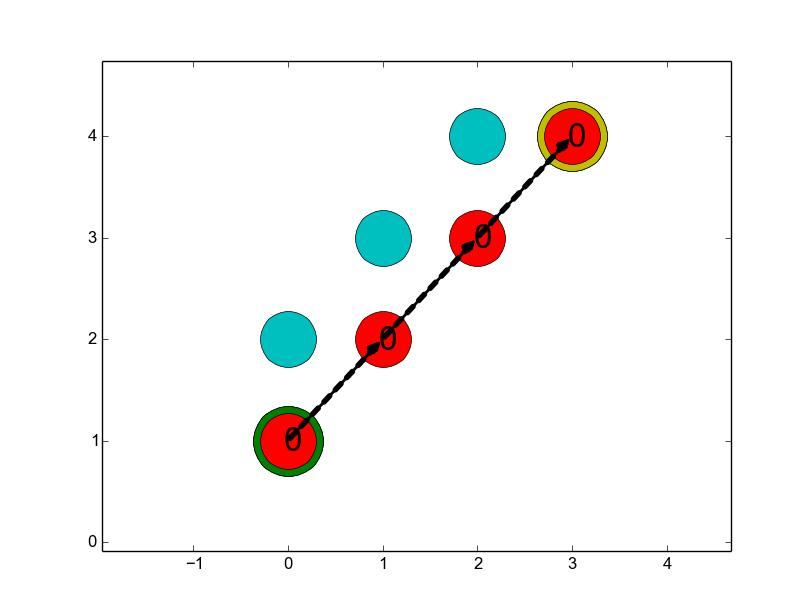
\includegraphics[scale=0.40]{./EJ2/todos0.png}
\\{\textit{Punteado = resultado exacto, contínua = resultado goloso}}
  \end{center}
  \vspace*{0.3cm}

Como se observa en el ejemplo el camino obtenido es exactamente el mismo.


\begin{center}
\textbf{Familia 4}
\end{center}

Se obtendr\'a la soluci\'on \'optima ya que, se reciben primero pokeparadas para vencer a un gimnasio cerca de ellas y luego m\'as pokeparadas para vencer a otros gimnasios que se encuentren cerca de estas \'ultimas, se mostrar\'a a continuaci\'on un dibujo que ejemplifica lo dicho:

\vspace*{0.3cm} \vspace*{0.3cm}
  \begin{center}
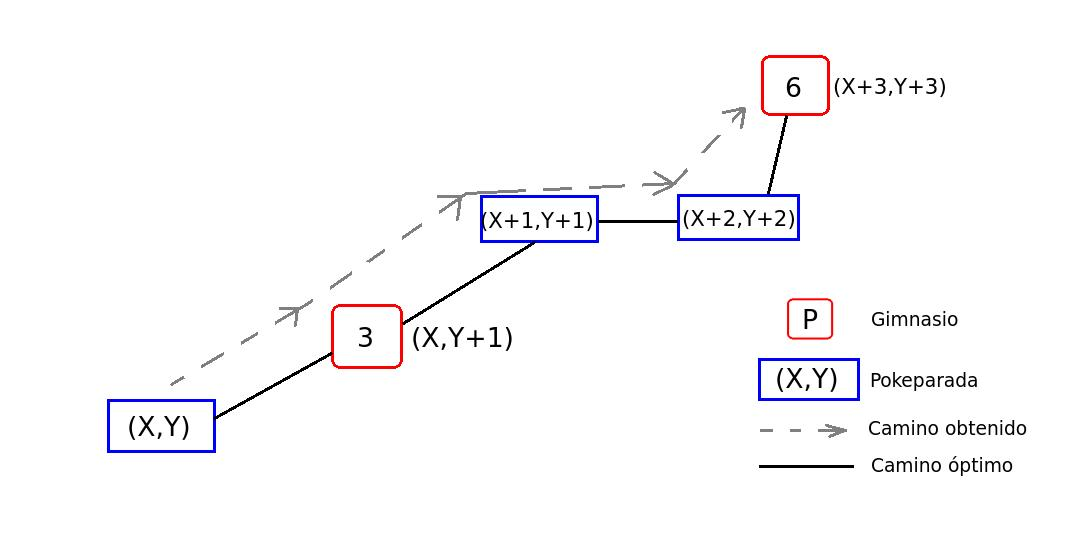
\includegraphics[scale=0.30]{./EJ2/optima.jpeg}
\\{\textit{Punteado = resultado exacto, contínua = resultado goloso}}
  \end{center}
  \vspace*{0.3cm}

\subsubsection*{Familia con soluci\'on no \'optima}

\begin{center}
\textbf{Familia 5}
\end{center}

Este estilo de familia se elabora de la forma en la cual existan gimnasios que no necesiten pociones para ser vencidos y otros que si. Nuestro algoritmo como por cada iteraci\'on chequea si puede elegir un gimnasio que se encuentre a una distancia m\'inima en relaci\'on a los demas, y adem\'as corrobora si posee las pociones necesarias para vencerlo, decide inicialmente ir a vencer a los gimnasios que posean cero poder, lo cual puede no ser \'optimo para el resultado final.

Debido al poder de computo, el algoritmo exacto solo puede tomar entre 20 o 25 elementos (dependiendo el tipo de instancia), mientras que el goloso puede tomar una mayor cantidad de elementos. Es por esto que se realizaron las comparaciones con la cantidad de elementos soportadas por el exacto.

A continuaci\'on un ejemplo comparativo entre ambos algoritmos con el cual se trabajo, dicho ejemplo contendr\'a un total de 21 elementos:



\begin{figure} [!ht]
 \centering
  \subfloat[Algoritmo exacto]{
    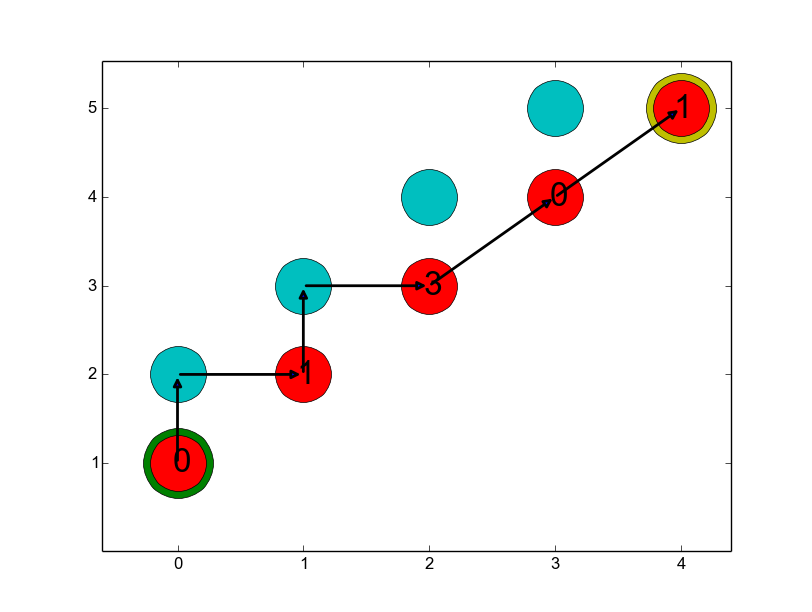
\includegraphics[width=0.45\textwidth]{./EJ2/fam5exacto.png}}
       \label{fig:jaggies}
  \subfloat[Algoritmo goloso]{
    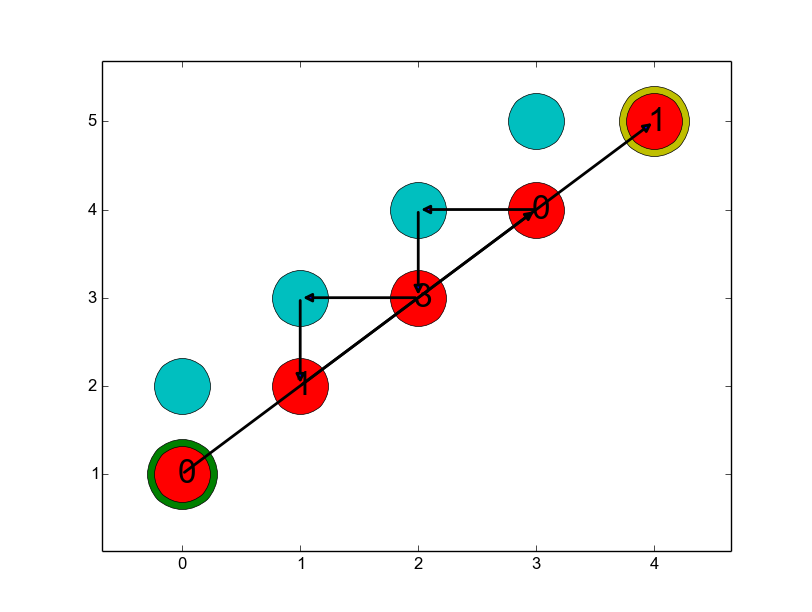
\includegraphics[width=0.45\textwidth]{./EJ2/fam5goloso.png}}
    \label{fig:moire}
    \end{figure}



Veremos a continuaci\'on en base a esta familia y el poder de computo cuanto ser\'a la diferencia de cada instancia de los algoritmos para luego calcular un porcentaje aproximado de la diferencia entre la soluci\'on obtenida del goloso y la \'optima.

\vspace*{0.3cm} \vspace*{0.3cm}
  \begin{center}
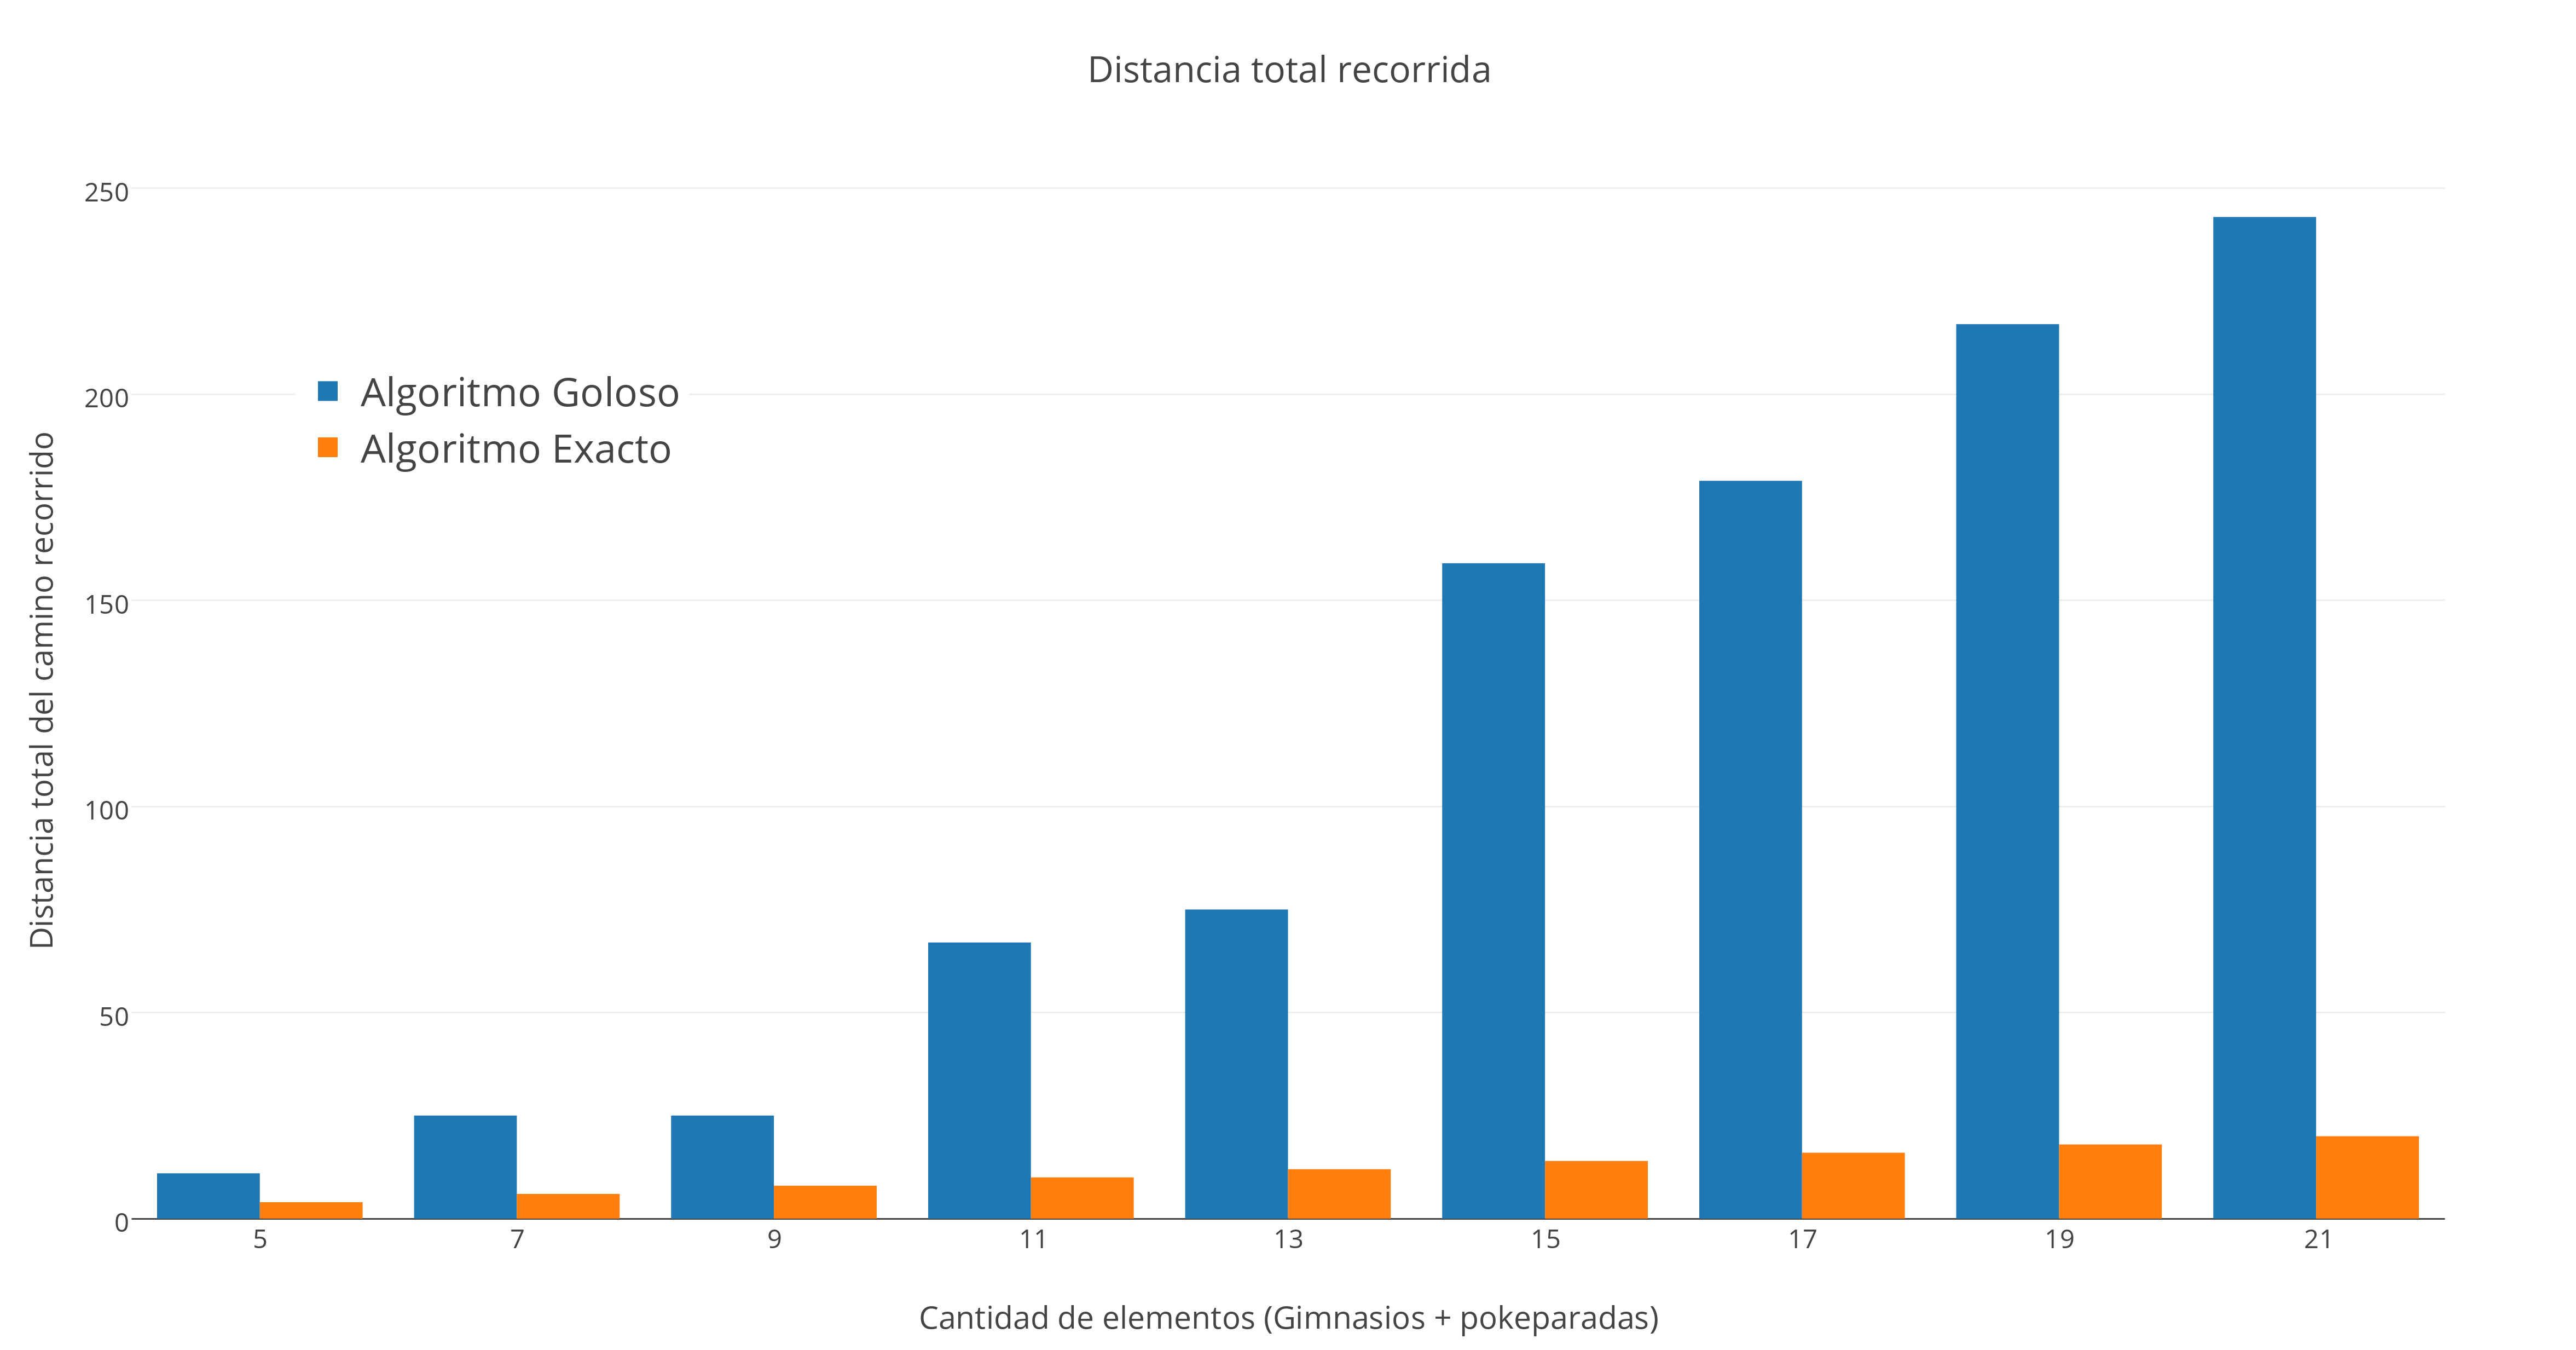
\includegraphics[scale=0.5]{./EJ2/algungym0.png}
\\{\textit{Ejemplo 2.7 Resultados obtenidos (Camino recorrido total) }}
  \end{center}
  \vspace*{0.3cm}


\begin{center}
\textbf{Familia 6}
\end{center}

Este estilo de familia presenta a los gimnasios y pokeparadas desordenados en referencia a las posiciones, es decir, para ganar a cierto gimnasio es necesario pasar por una cantidad puntual de pokeparadas las cuales estan de un lado y del otro de dicho gimnasio.
(VER DE ESCRIBIR ESTO MAS EN DETALLE)

\vspace*{0.3cm} \vspace*{0.3cm}
  \begin{center}
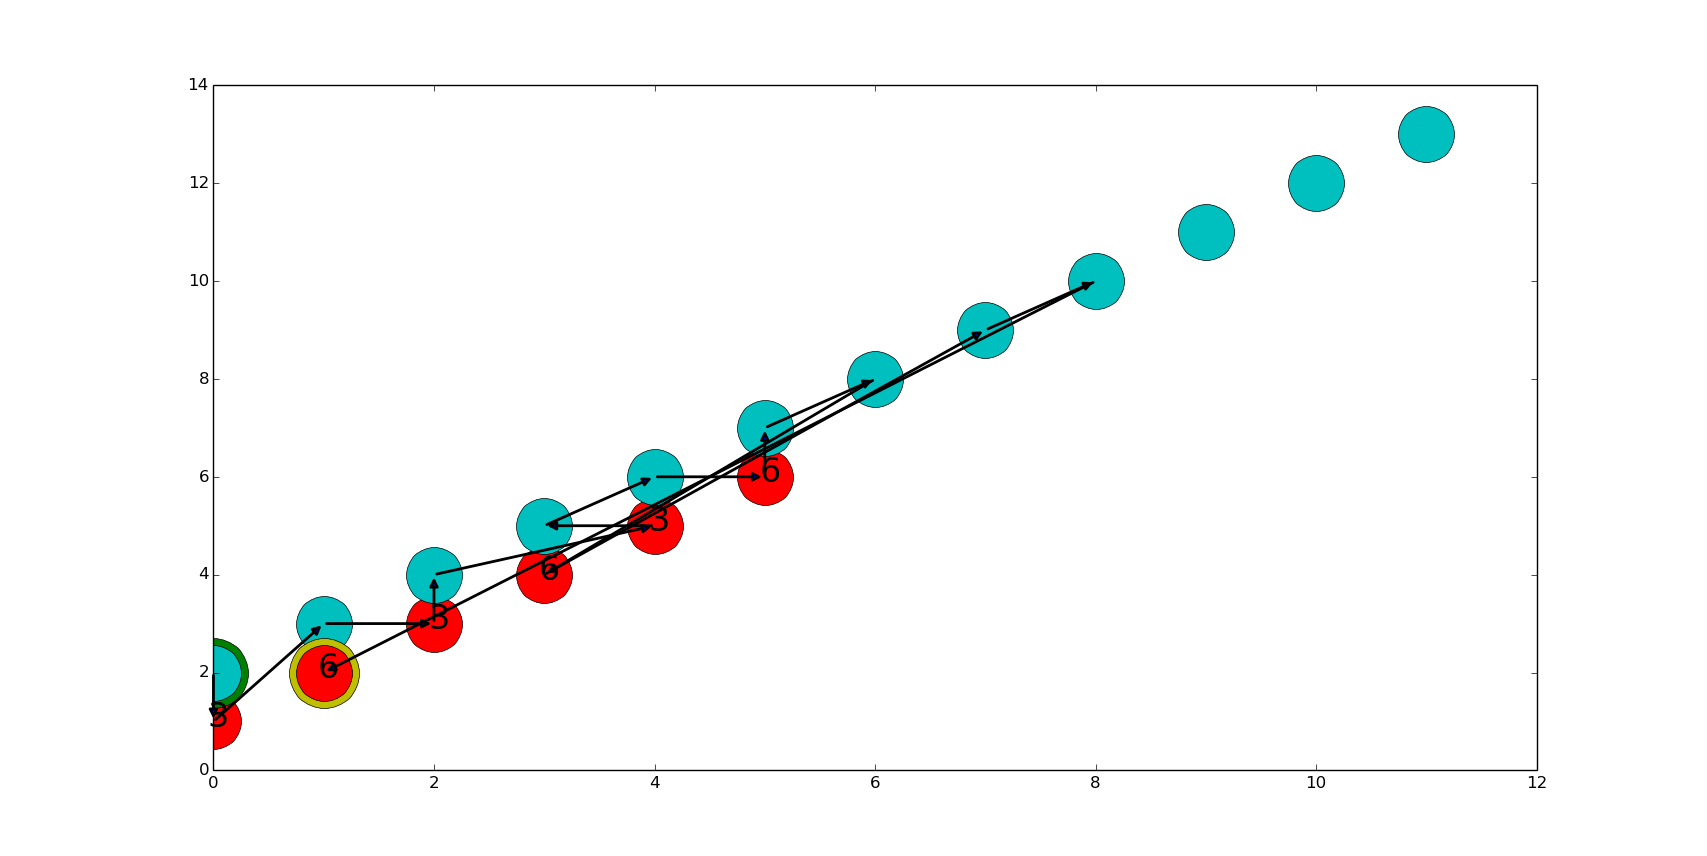
\includegraphics[scale=0.40]{./EJ2/caminosinorden1.png}
\\{\textit{Ejemplo 2.5 Resultados obtenidos - Algoritmo Goloso}}
  \end{center}
  \vspace*{0.3cm}
  
\vspace*{0.3cm} \vspace*{0.3cm}
  \begin{center}
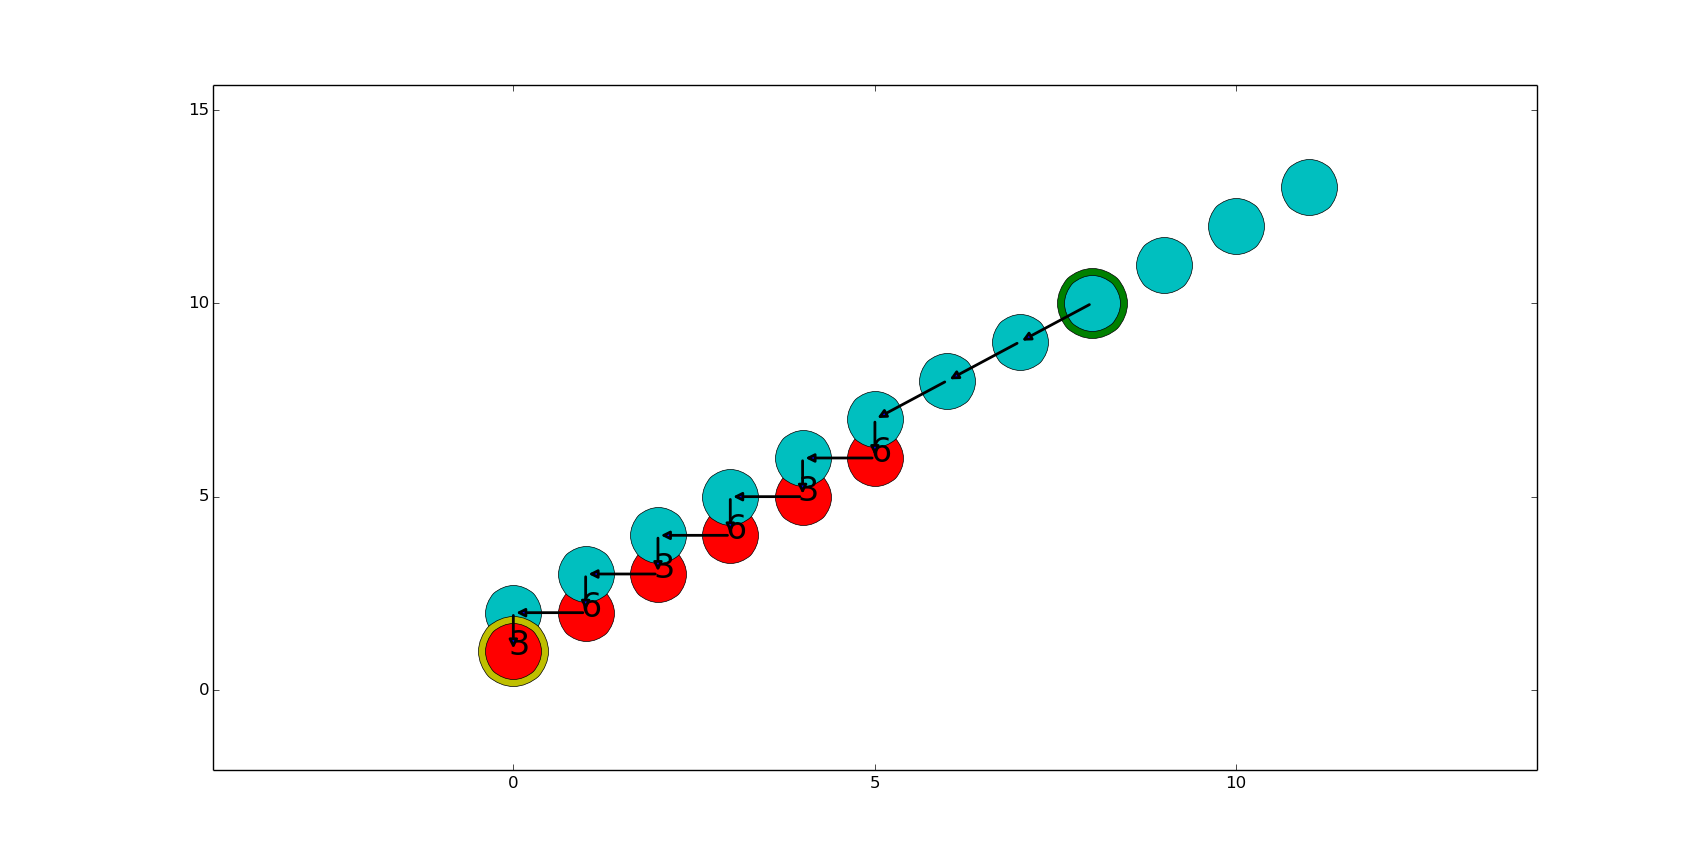
\includegraphics[scale=0.40]{./EJ2/caminosinorden.png}
\\{\textit{Ejemplo 2.6 Resultados obtenidos - Algoritmo Exacto}}
  \end{center}
  \vspace*{0.3cm}

Se puede observar en el ejemplo 2.5 como nuestro algorimo va a la primer pokeparada y de ah\'i va a vencer al gimnasio m\'as cercano en vez de ir a la pokeparada que se encuentra inmediatamente consecutiva. Esto lo hace hasta vencer a todos los gimnasios.

A continuacion mostraremos para cada instancia posible de ser comparada el error obtenido en cada soluci\'on:

\vspace*{0.3cm} \vspace*{0.3cm}
  \begin{center}
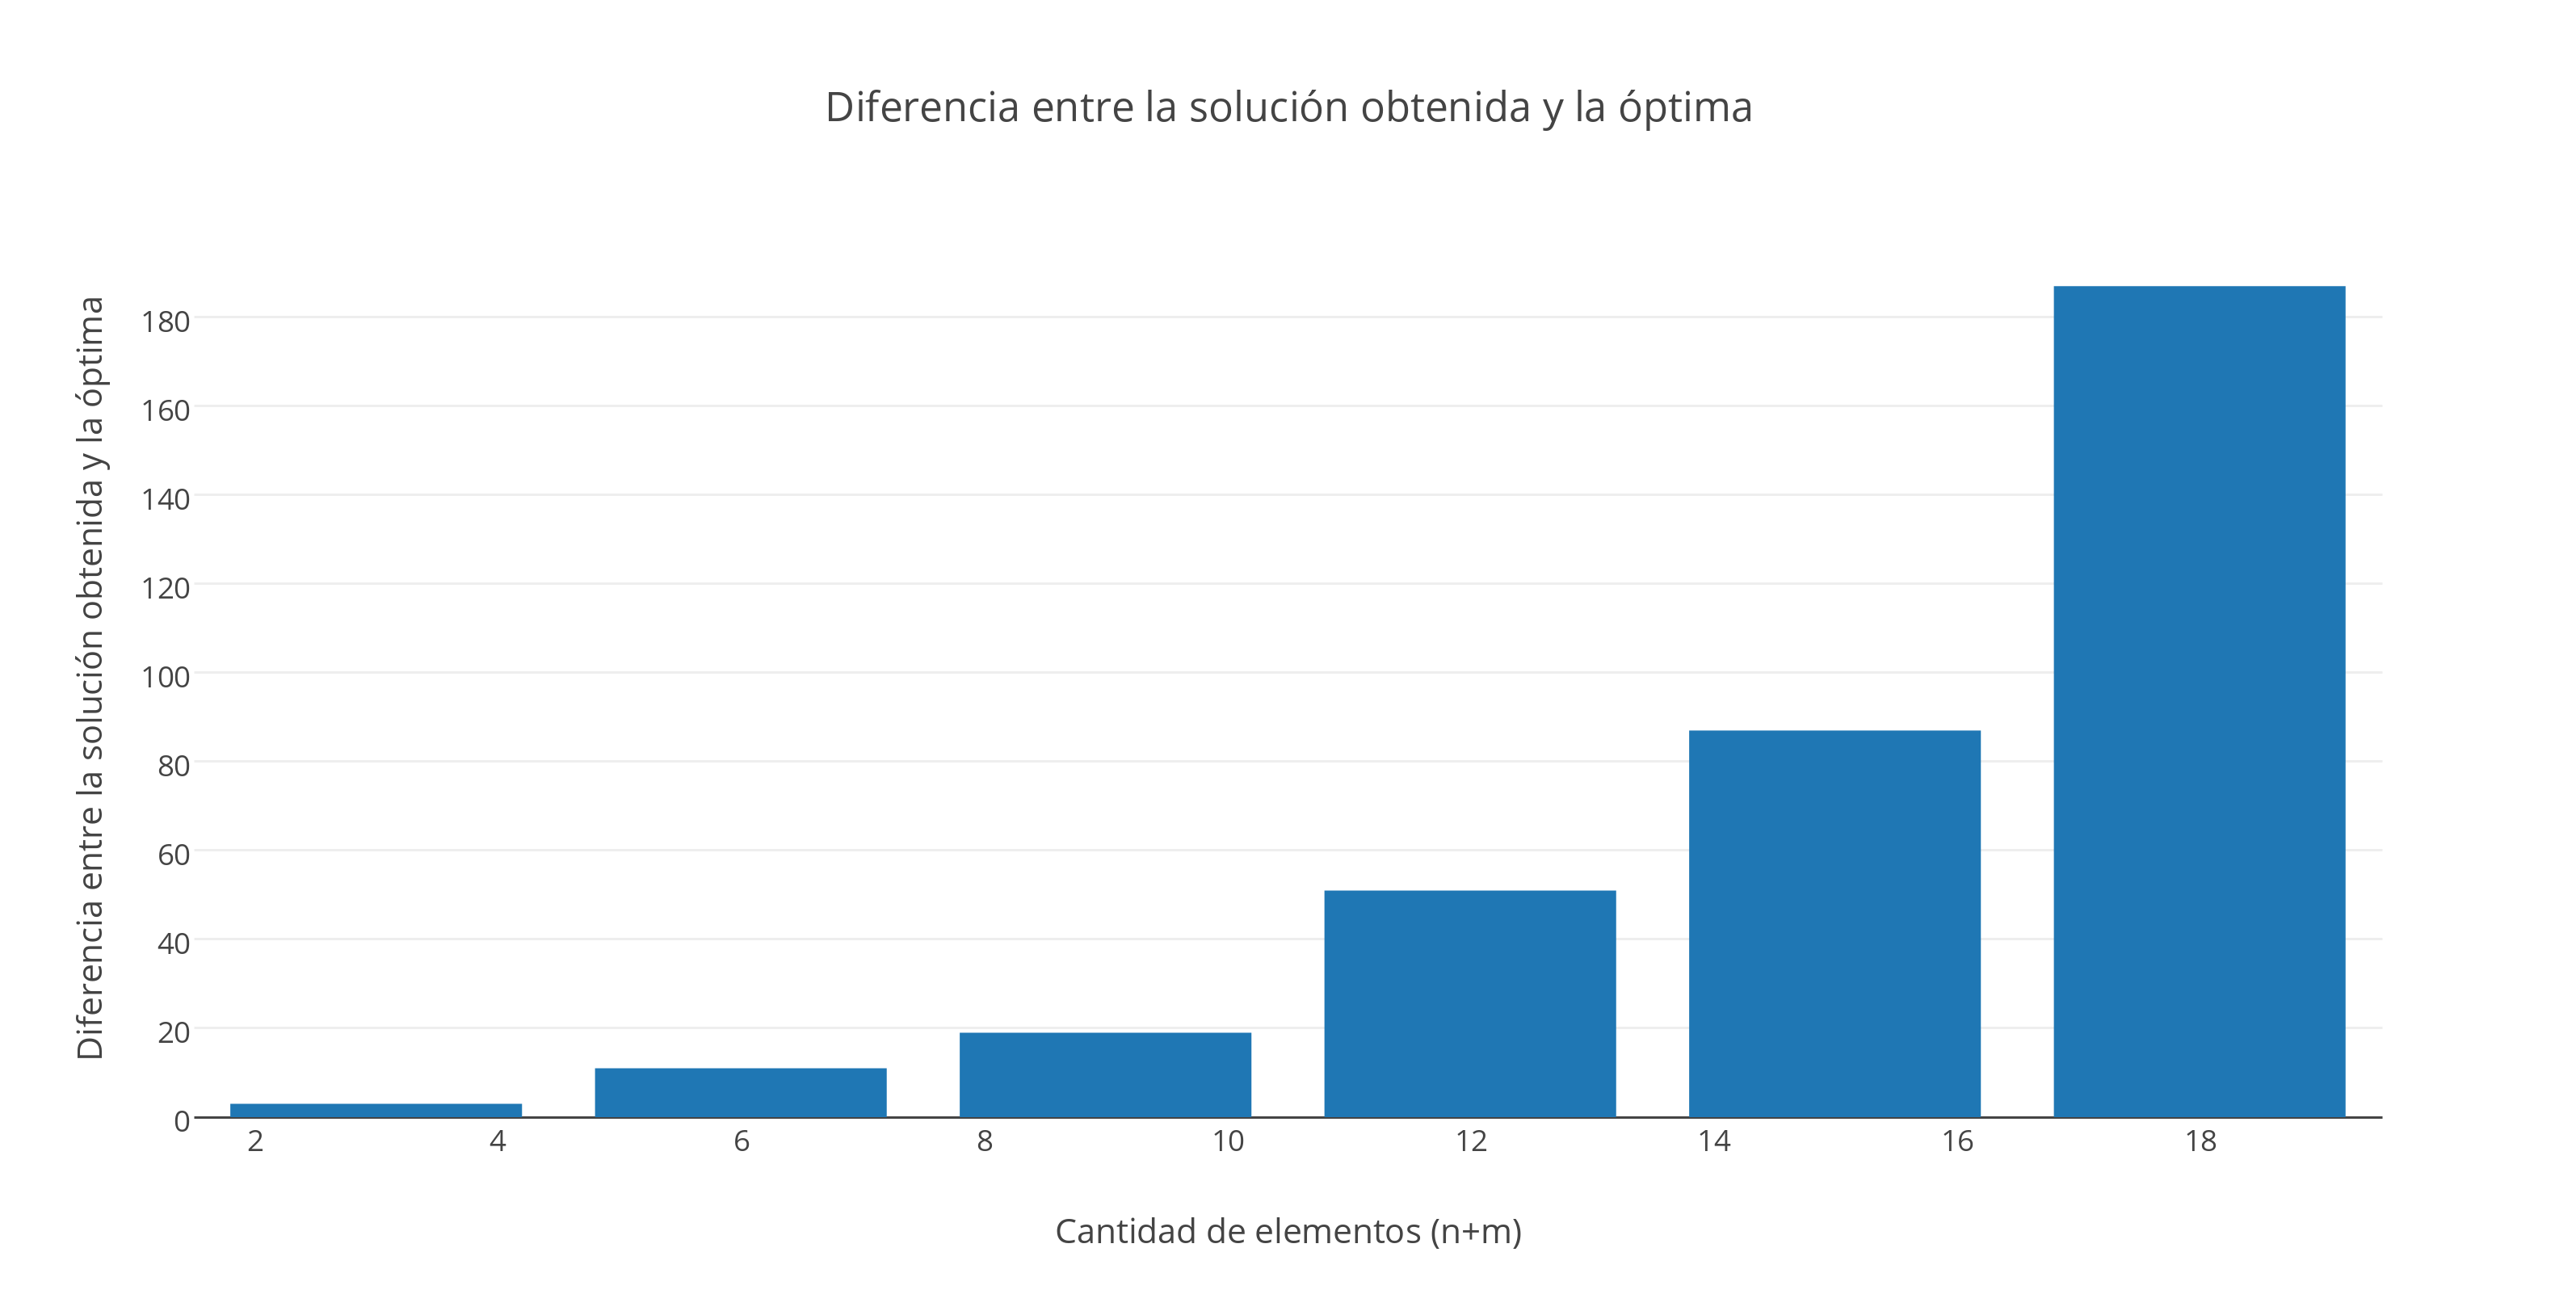
\includegraphics[scale=0.40]{./EJ2/sinOrden.png}
\\{\textit{Ejemplo 2.7 Resultados obtenidos (Camino recorrido total) }}
  \end{center}
  \vspace*{0.3cm}
  
\begin{center}
\textbf{Familia 7}
\end{center}

Este estilo de familia se elabora de la forma en la cual se tengan todos los gimnasios en ciertas posiciones, donde el conjunto total de estos nos devuelva una forma de anillo, mientras que las pokeparadas presenten la misma forma que los gimnasios a una distancia euclidea id\'entica entre pokeparada-gimnasio. Como mencionamos nuestro algoritmo siempre que puede vencer a alg\'un gimnasio busca cual es el m\'inimo en relaci\'on a la distancia y va a vencerlo, lo cual en este caso puntual ser\'a contraproducente ya que es preferible adquirir m\'as pociones para luego ir a varios gimnasios juntos. (ESTO HABRIA QUE REESCRIBIRLO PORQUE NO QUEDA MUY CLARO)

\begin{figure} [!ht]
 \centering
  \subfloat[Algoritmo exacto]{
    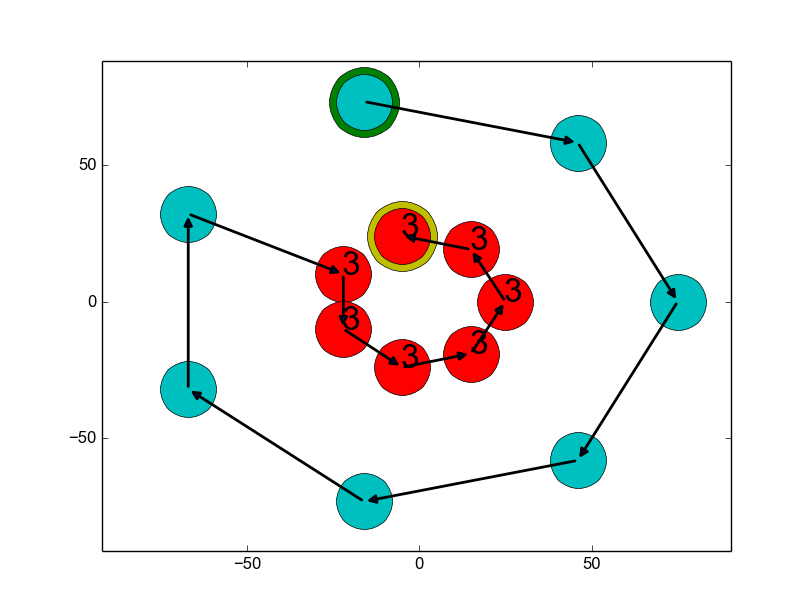
\includegraphics[width=0.45\textwidth]{./EJ2/anilloexacto.png}}
       \label{fig:jaggies}
  \subfloat[Algoritmo goloso]{
    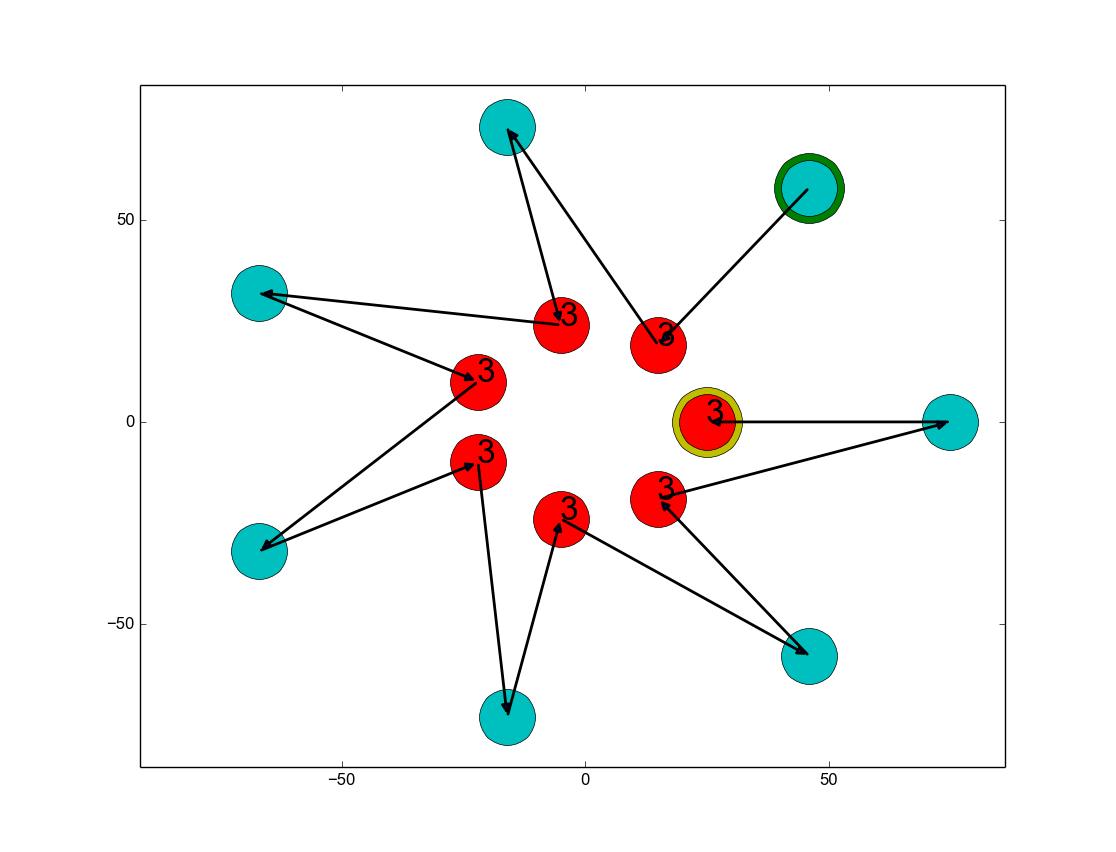
\includegraphics[width=0.45\textwidth]{./EJ2/anillogoloso.png}}
    \label{fig:moire}
    \end{figure}

A continuacion mostraremos para cada instancia posible de ser comparada el error obtenido en cada soluci\'on:

\vspace*{0.3cm} \vspace*{0.3cm}
  \begin{center}
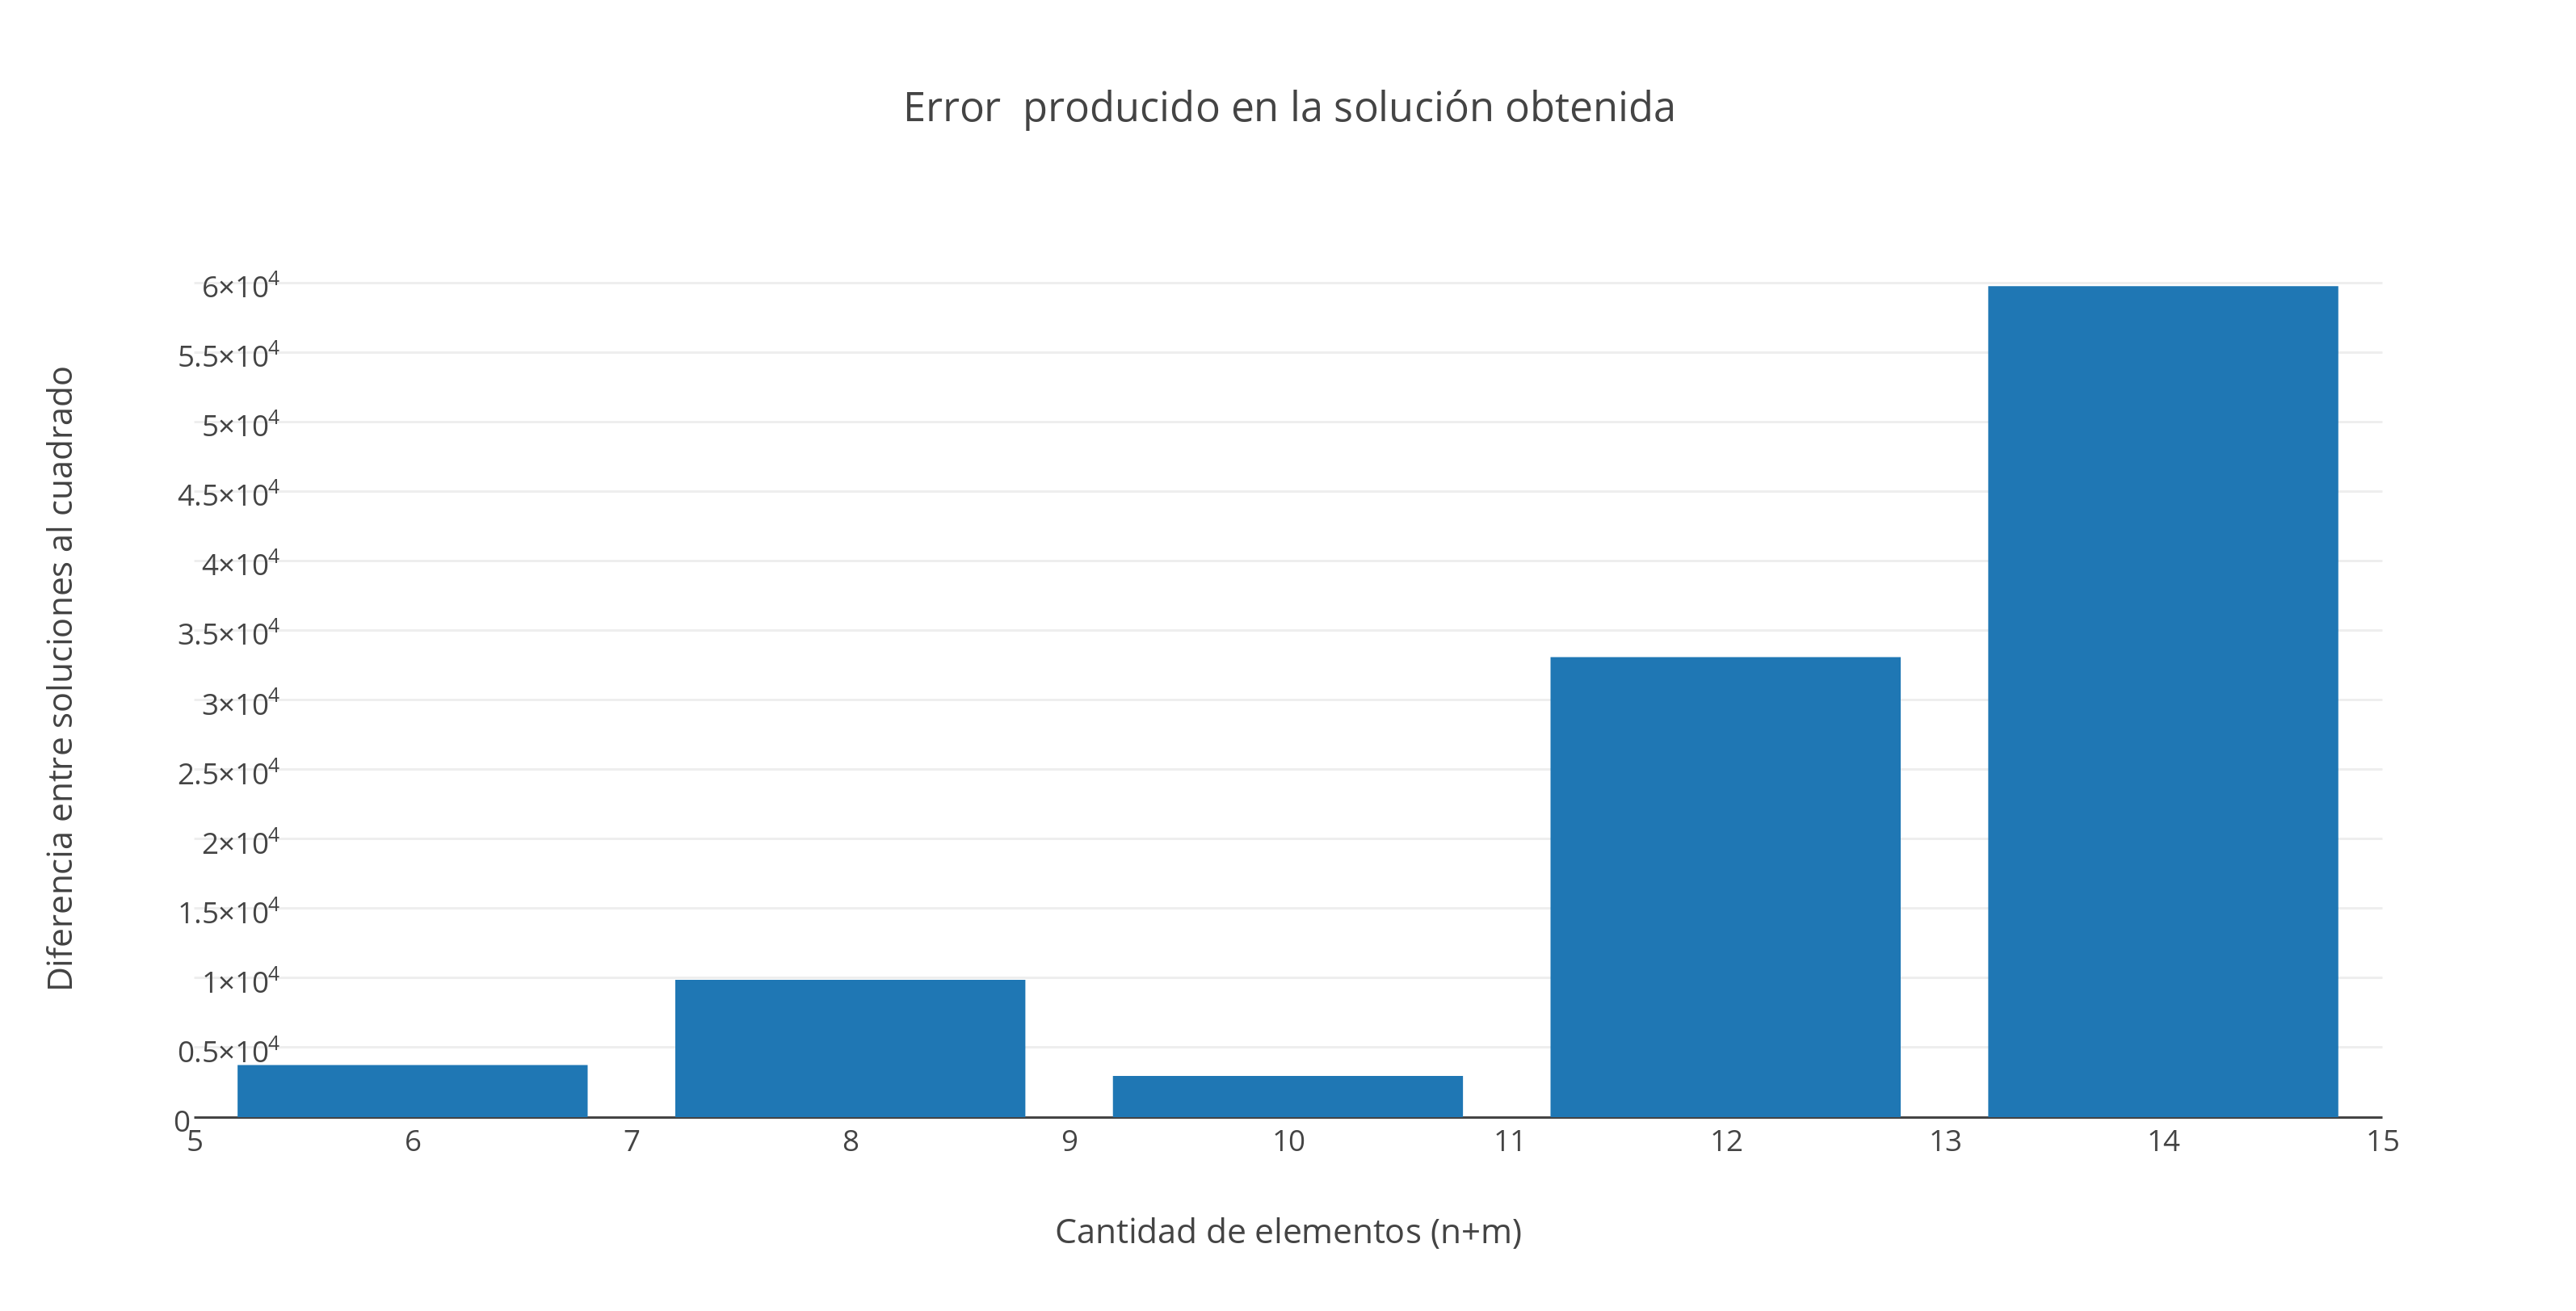
\includegraphics[scale=0.40]{./EJ2/anillosdif.png}
\\{\textit{Ejemplo 2.7 Resultados obtenidos (Camino recorrido total) }}
  \end{center}
  \vspace*{0.3cm}
  
  
Por \'ultimo, la familia sin soluci\'on \'optima n\'umero 8 la cual es random.


\begin{figure} [!ht]
 \centering
  \subfloat[Algoritmo exacto]{
    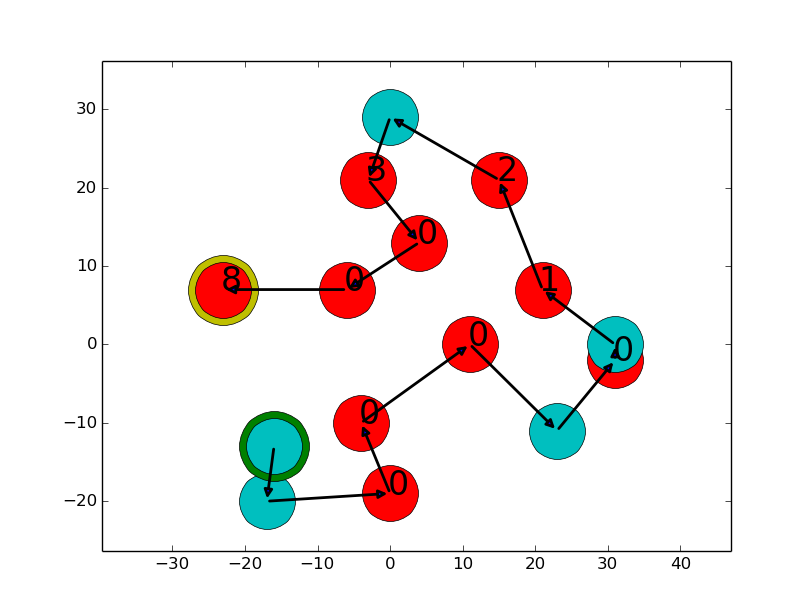
\includegraphics[width=0.45\textwidth]{./EJ2/randomexacto.png}}
       \label{fig:jaggies}
  \subfloat[Algoritmo goloso]{
    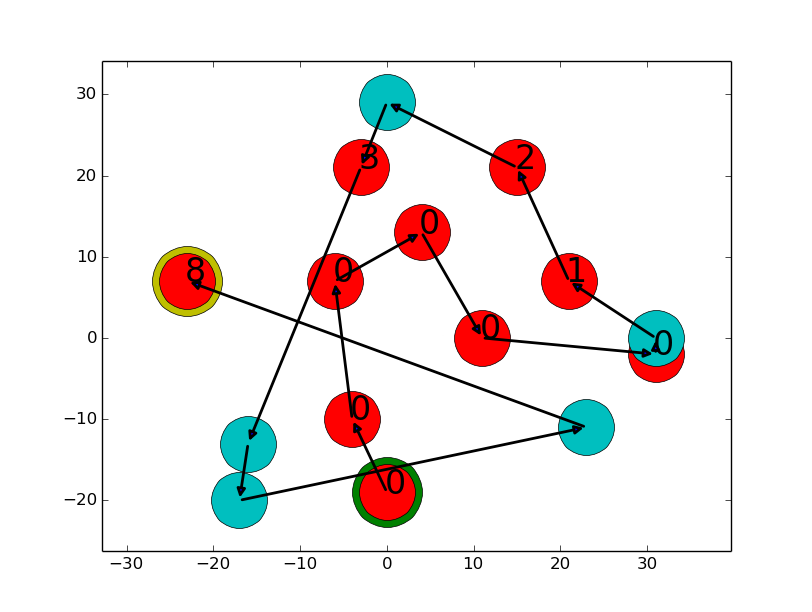
\includegraphics[width=0.45\textwidth]{./EJ2/randomgoloso.png}}
    \label{fig:moire}
    \end{figure}

A continuacion mostraremos para cada instancia posible de ser comparada el error obtenido en cada soluci\'on:

\vspace*{0.3cm} \vspace*{0.3cm}
  \begin{center}
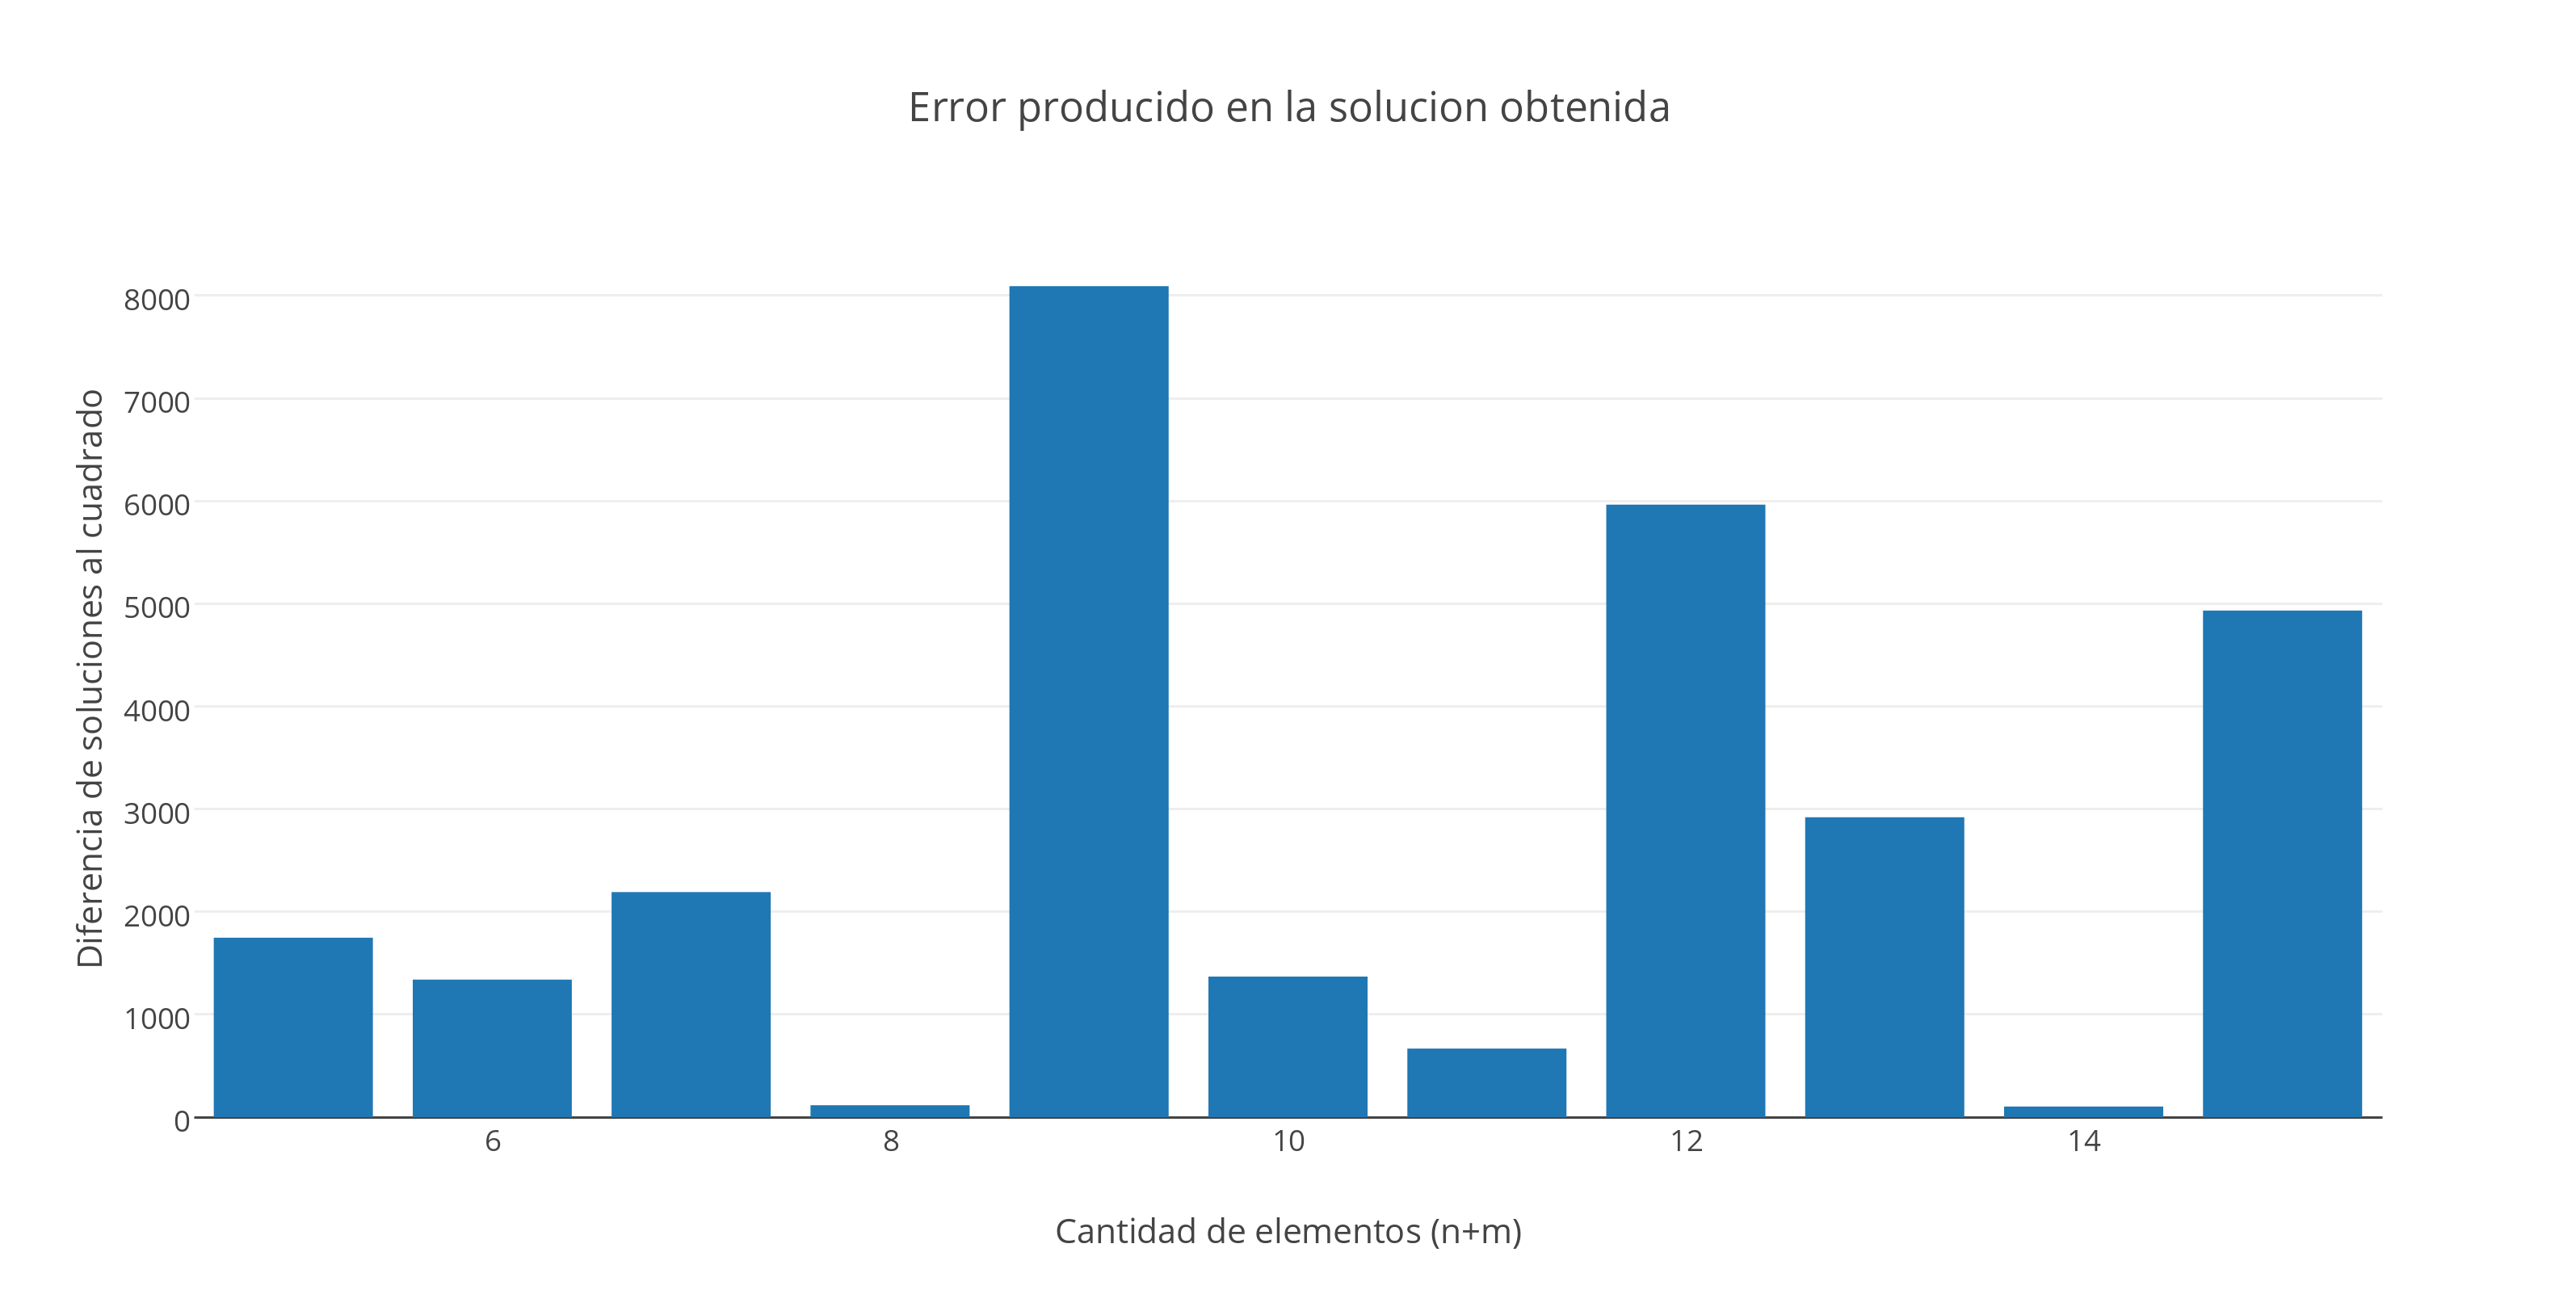
\includegraphics[scale=0.40]{./EJ2/randomdif.png}
\\{\textit{Ejemplo 2.7 Resultados obtenidos (Camino recorrido total) }}
  \end{center}
  \vspace*{0.3cm}
  

Luego de lo comentado mostraremos dos gr\'aficos con los errores producidos por cada familia en la soluci\'on obtenida.

\vspace*{0.3cm} \vspace*{0.3cm}
  \begin{center}
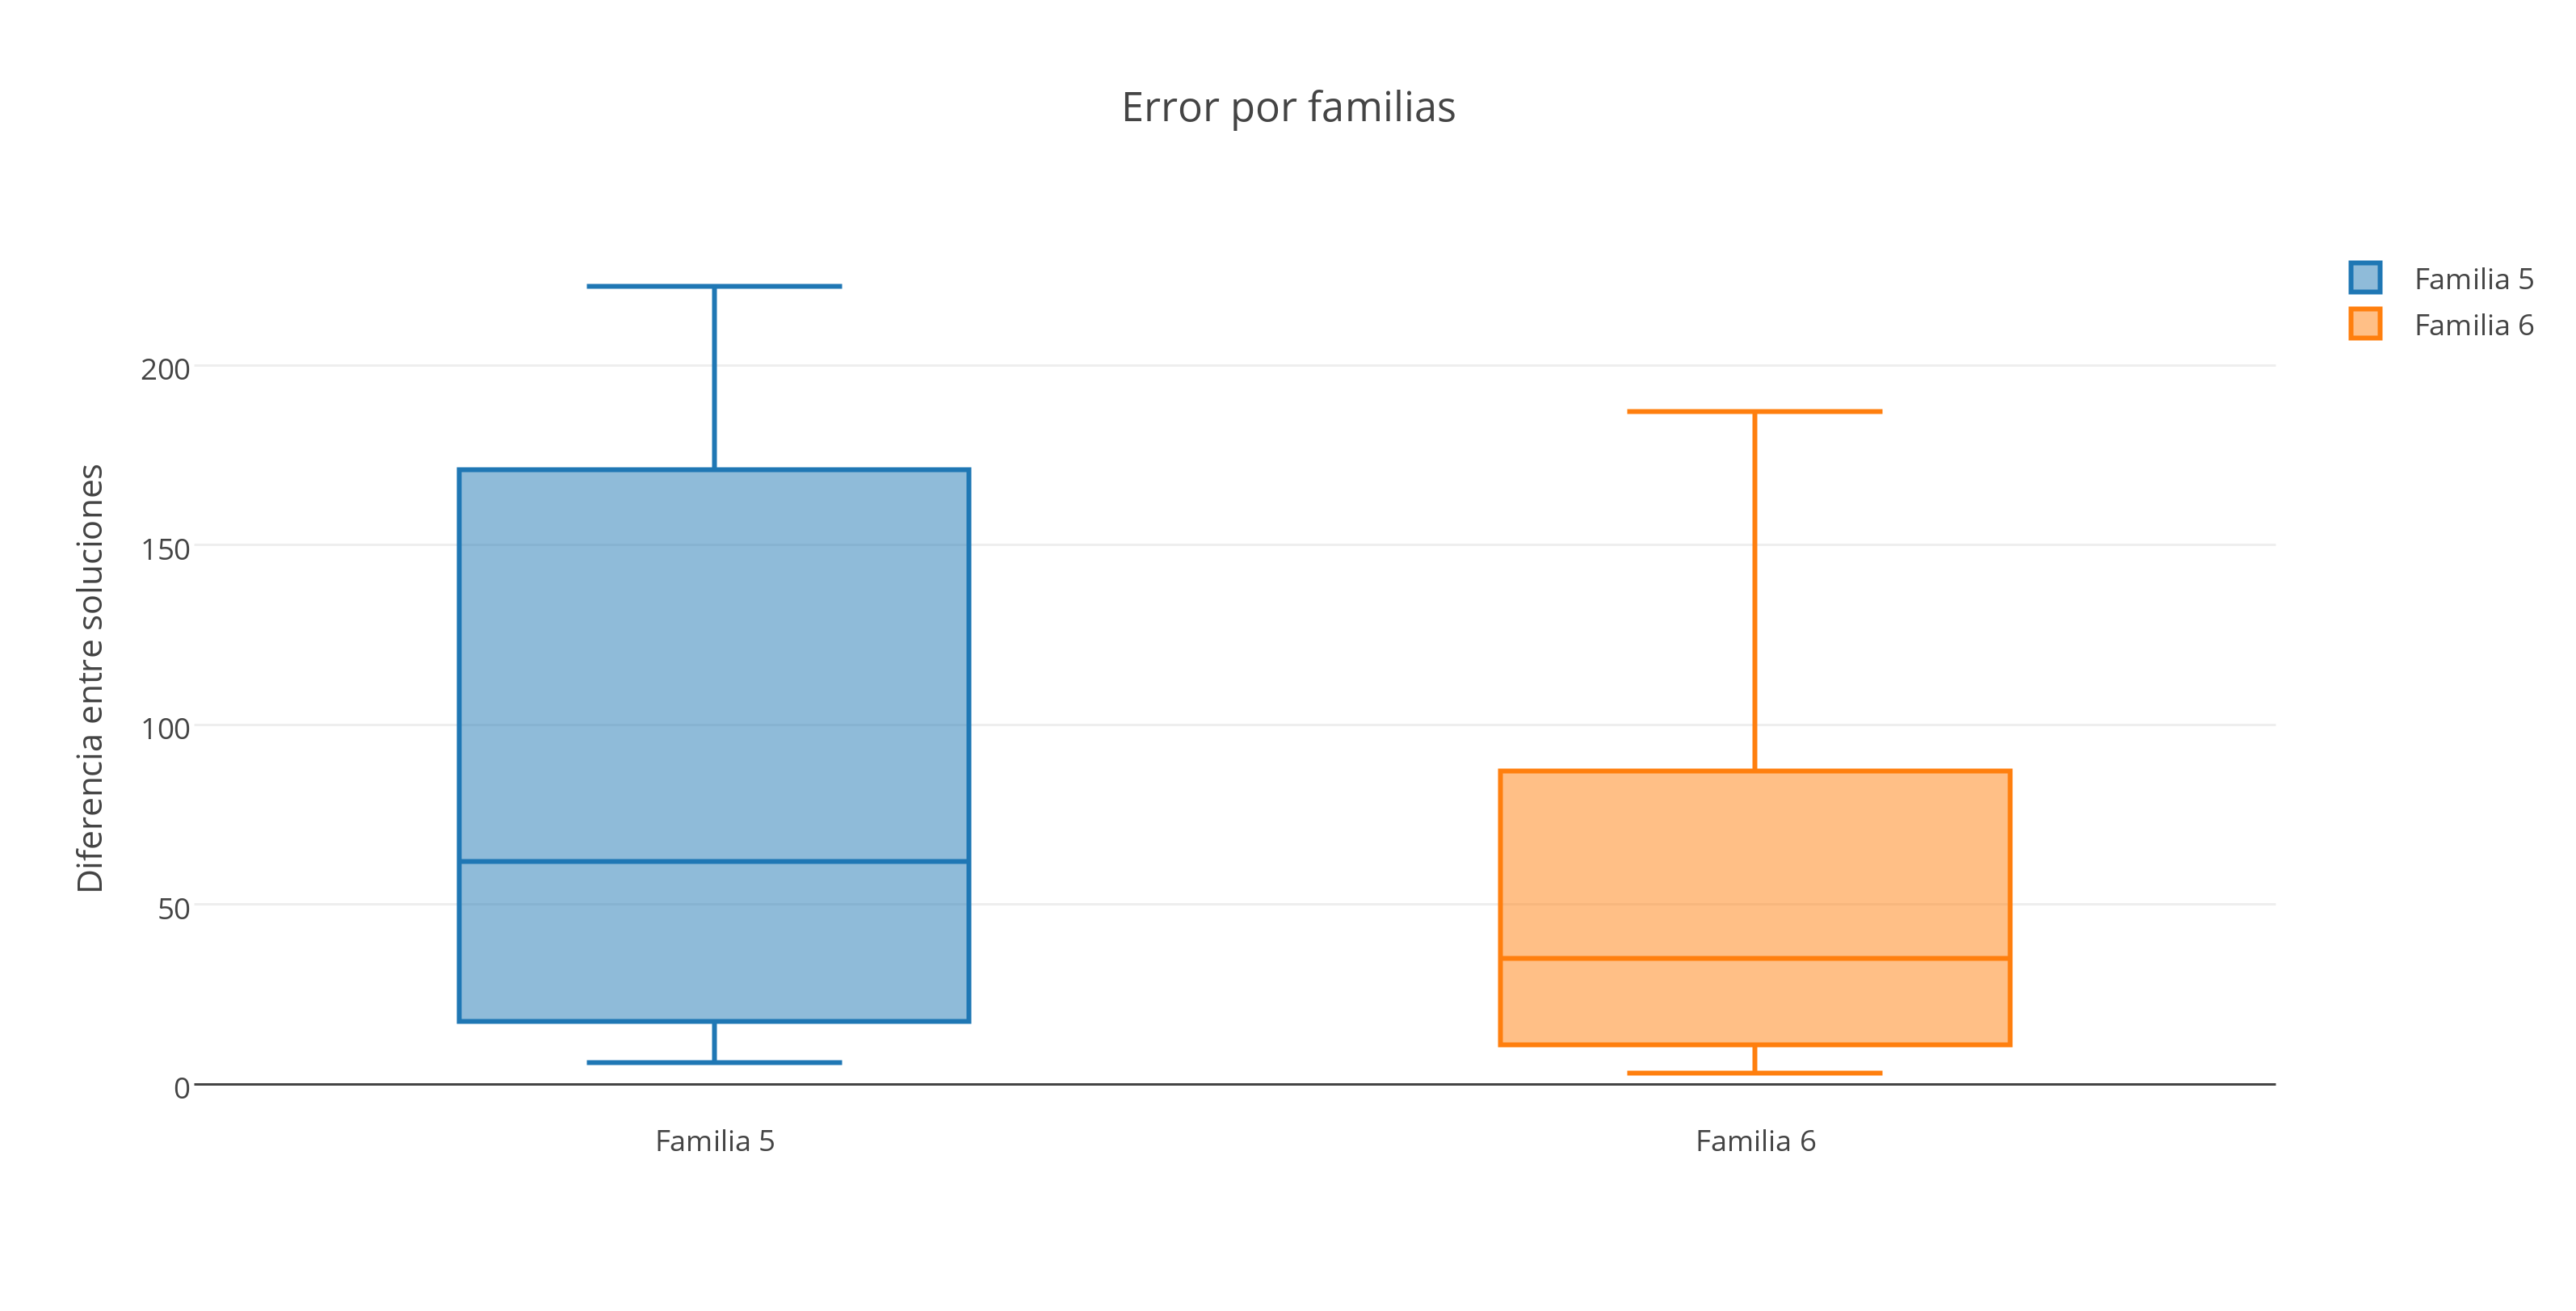
\includegraphics[scale=0.60]{./EJ2/box1.png}
\\{\textit{Familia 5 y 6 error de solucion}}
  \end{center}
  \vspace*{0.3cm}
  
\vspace*{0.3cm} \vspace*{0.3cm}
  \begin{center}
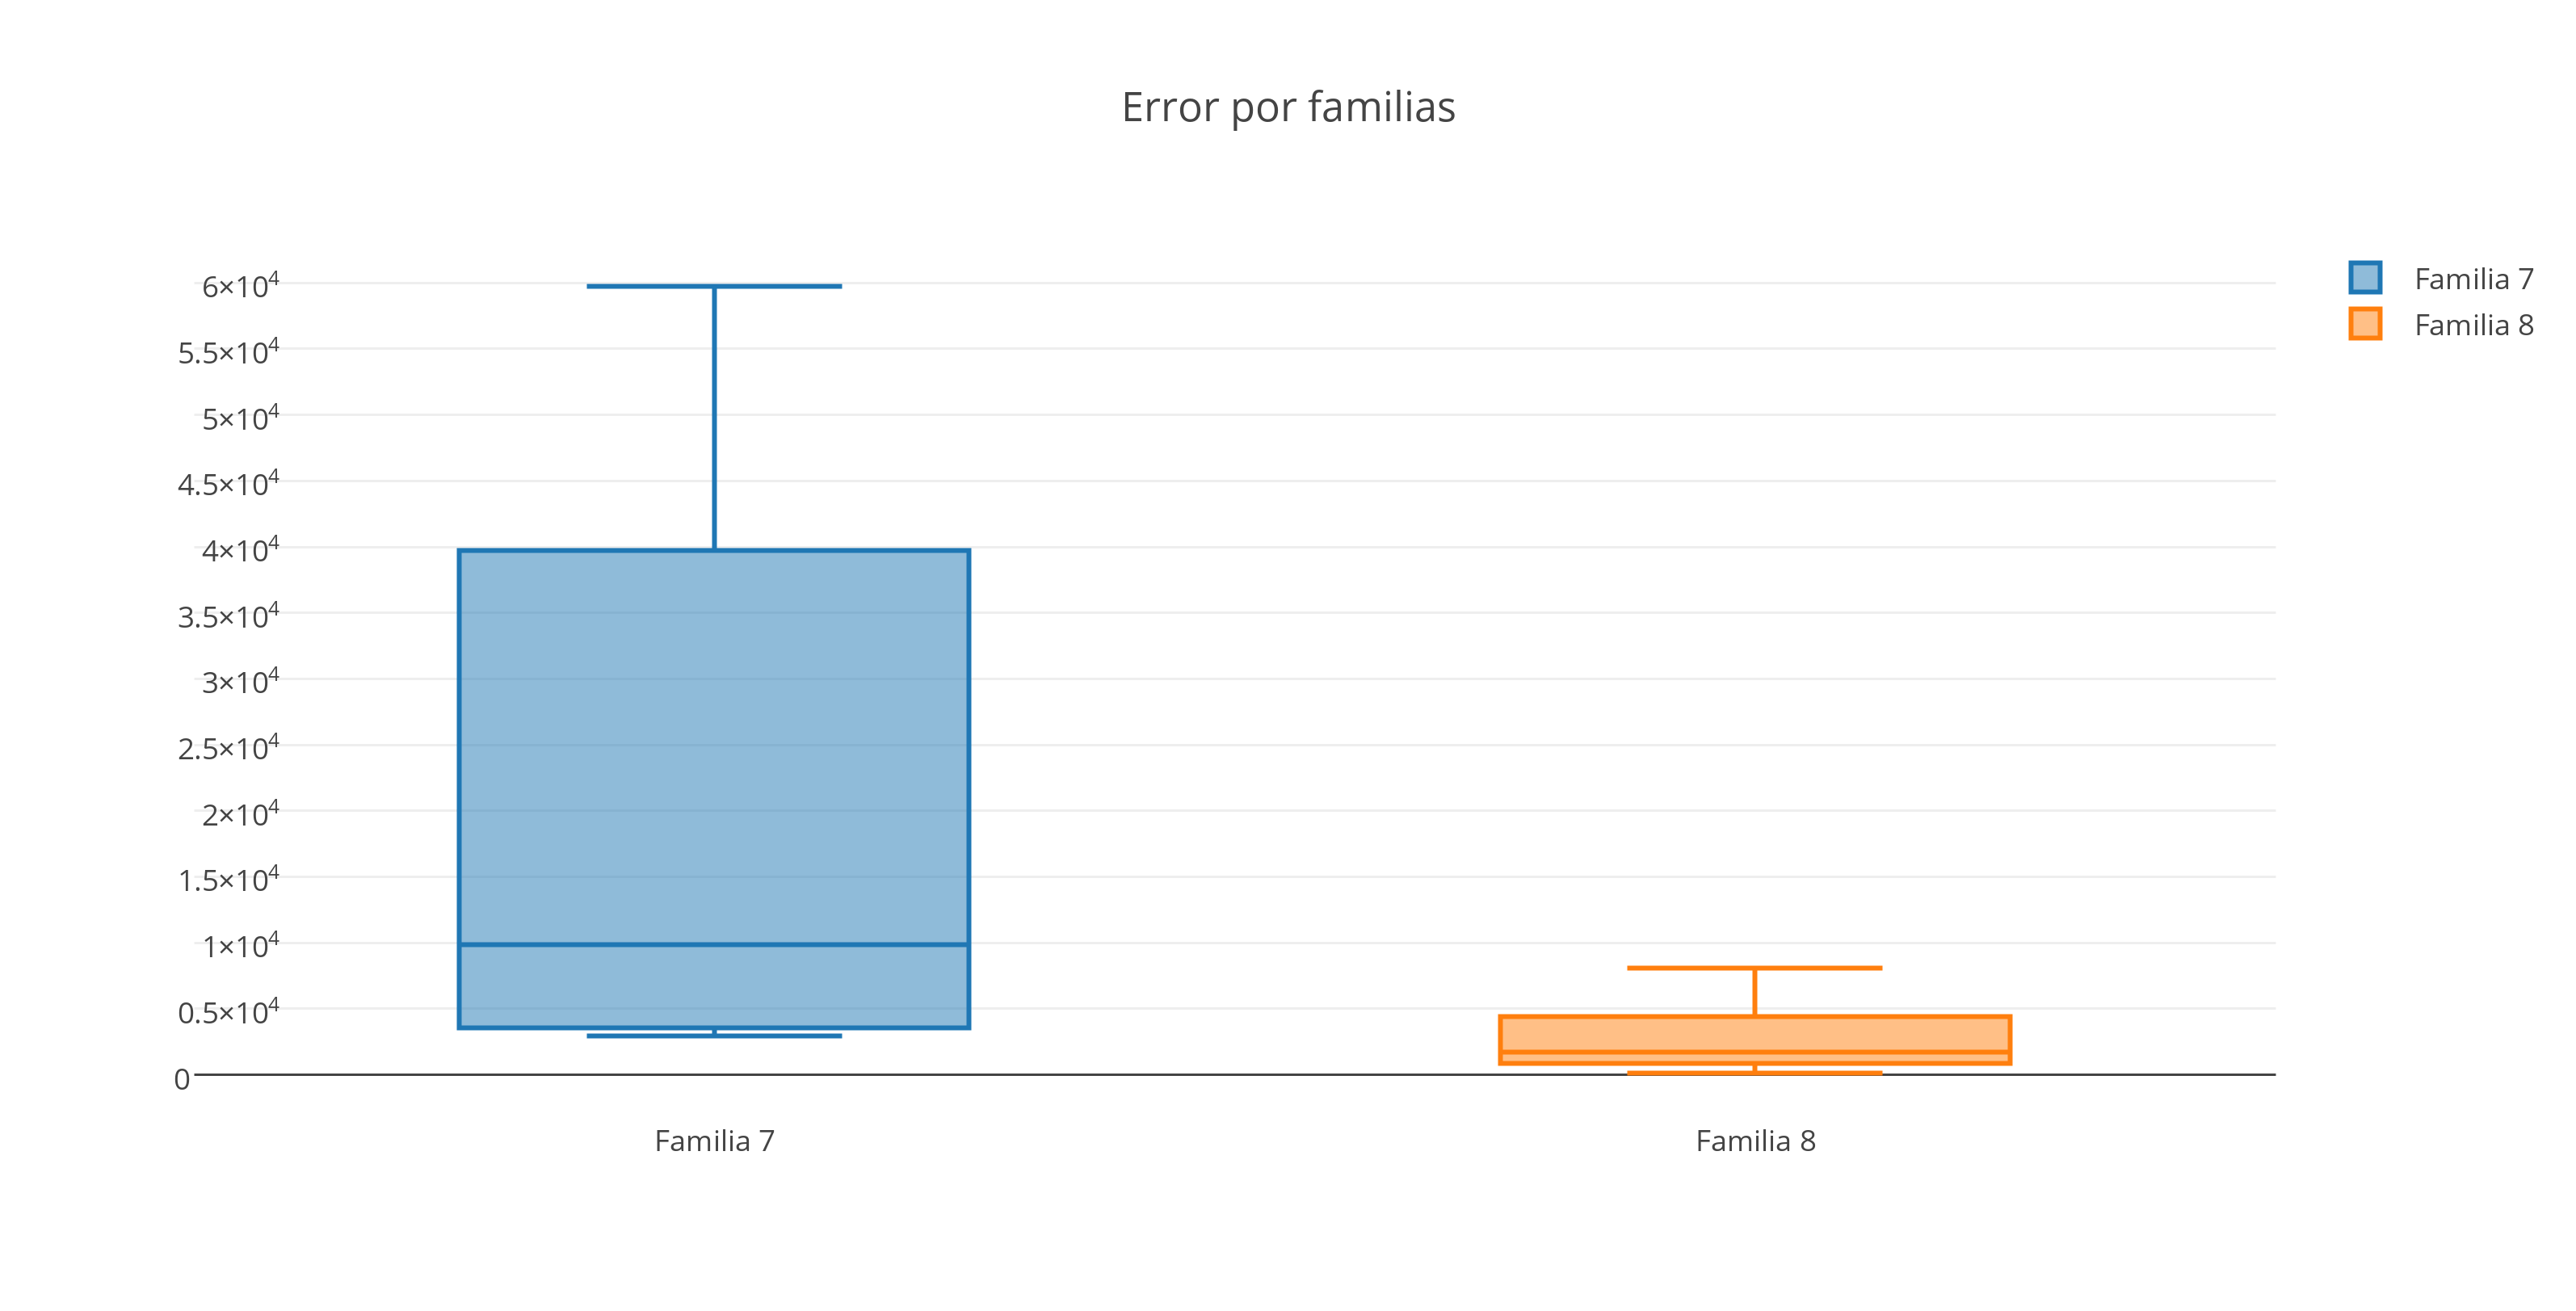
\includegraphics[scale=0.60]{./EJ2/box2.png}
\\{\textit{Familia 7 y 8 error de solucion}}
  \end{center}
  \vspace*{0.3cm}
  
En conclusi\'on, la soluci\'on obtenida distará tanto de la óptima como la cantidad de veces que el algoritmo recorra una pokeparada y luego un gimnasio a vencerlo, sin importar si lo optimo era pasar primero por las pokeparadas juntando poder y luego visitar varios gimnasios consecutivamente venciendolos a todos.
El peor caso será cuando el mapa sea un anillo de pokeparadas con un anillo interno o externo de gimnasios. 
El algoritmo iniciará en una pokeparada, luego irá a ganar a un gimansio con distancia mínima dentro de los gimansios no visitados, y siguiendo este recorrido, volverá a una pokeparada que se encuentre a una distancia menor de la pokeparada previa.\\

Posteriormente, veremos como se comporta cada familia en funcion del tiempo al ir aumentando la cantidad de elementos manteniendo las condiciones para que sigan perteneciendo cada uno a su respectiva familia.

\vspace*{0.3cm} \vspace*{0.3cm}
  \begin{center}
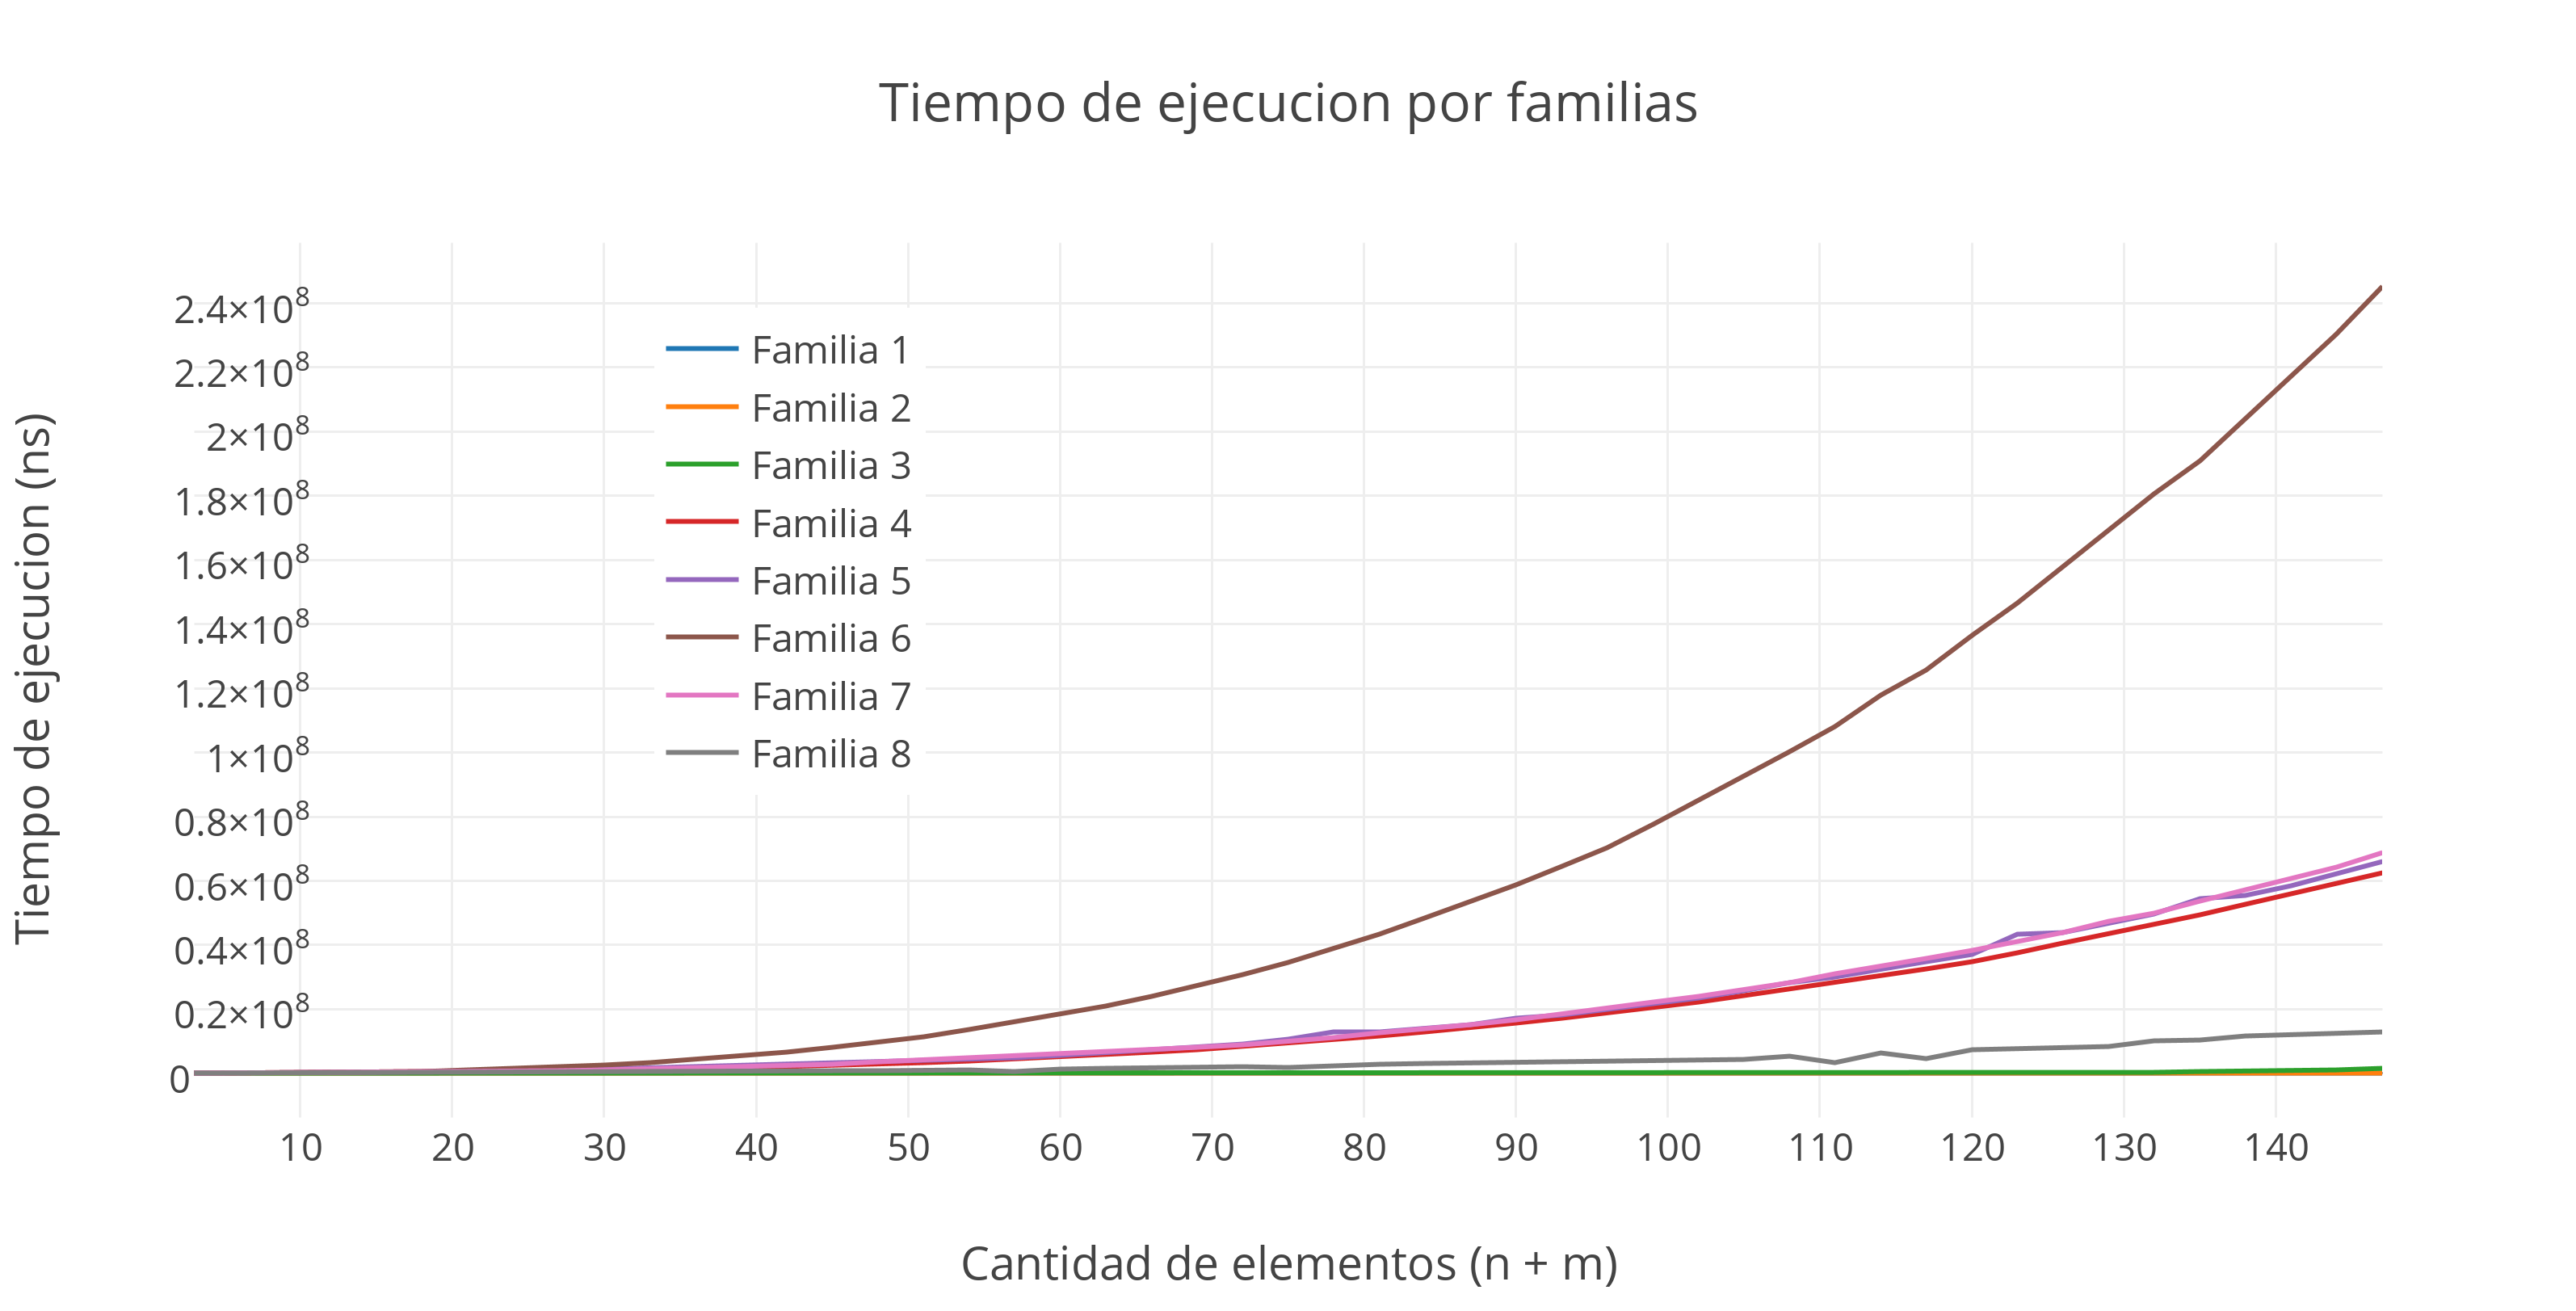
\includegraphics[scale=0.60]{./EJ2/comparativo.png}
\\{\textit{Tiempo de ejecución entre familias}}
  \end{center}
  \vspace*{0.3cm}
  
Se puede observar como la familia n\'umero 6 presenta una peor performance en comparaci\'on al resto mientras que tanto la familia 1 como la 2 presentan un tiempo que se torna constante dando una mejor performance en relaci\'on al resto, lo cual se debe a las podas utilizadas para estas familias como mencionamos anteriormente. Mientras que la n\'umero 6 presenta la dificultad en la cual todos los elementos del mapa se encuentran desordenados, por lo tanto nuestro algoritmo tiene que llegar a hacer hasta un doble viaje para poder vencer a un gimnasio, ya que se dan instancias en las cuales los gimnasios de poder menor o igual a 3 se encuentran muy lejos de las pokeparadas en relaci\'on a los gimnasios de poder mayor los cuales estan "pegados" a las pokeparadas insumiendole as\'i un tiempo mayor de decisi\'on y ejecuci\'on. Como hab\'iamos visto, nuestro algoritmo siempre que puede vencer a un gimnasio va a vencerlo.

Luego, mostraremos como se comporta nuestro algoritmo en base a la complejidad calculada anteriormente:

\vspace*{0.3cm} \vspace*{0.3cm}
  \begin{center}
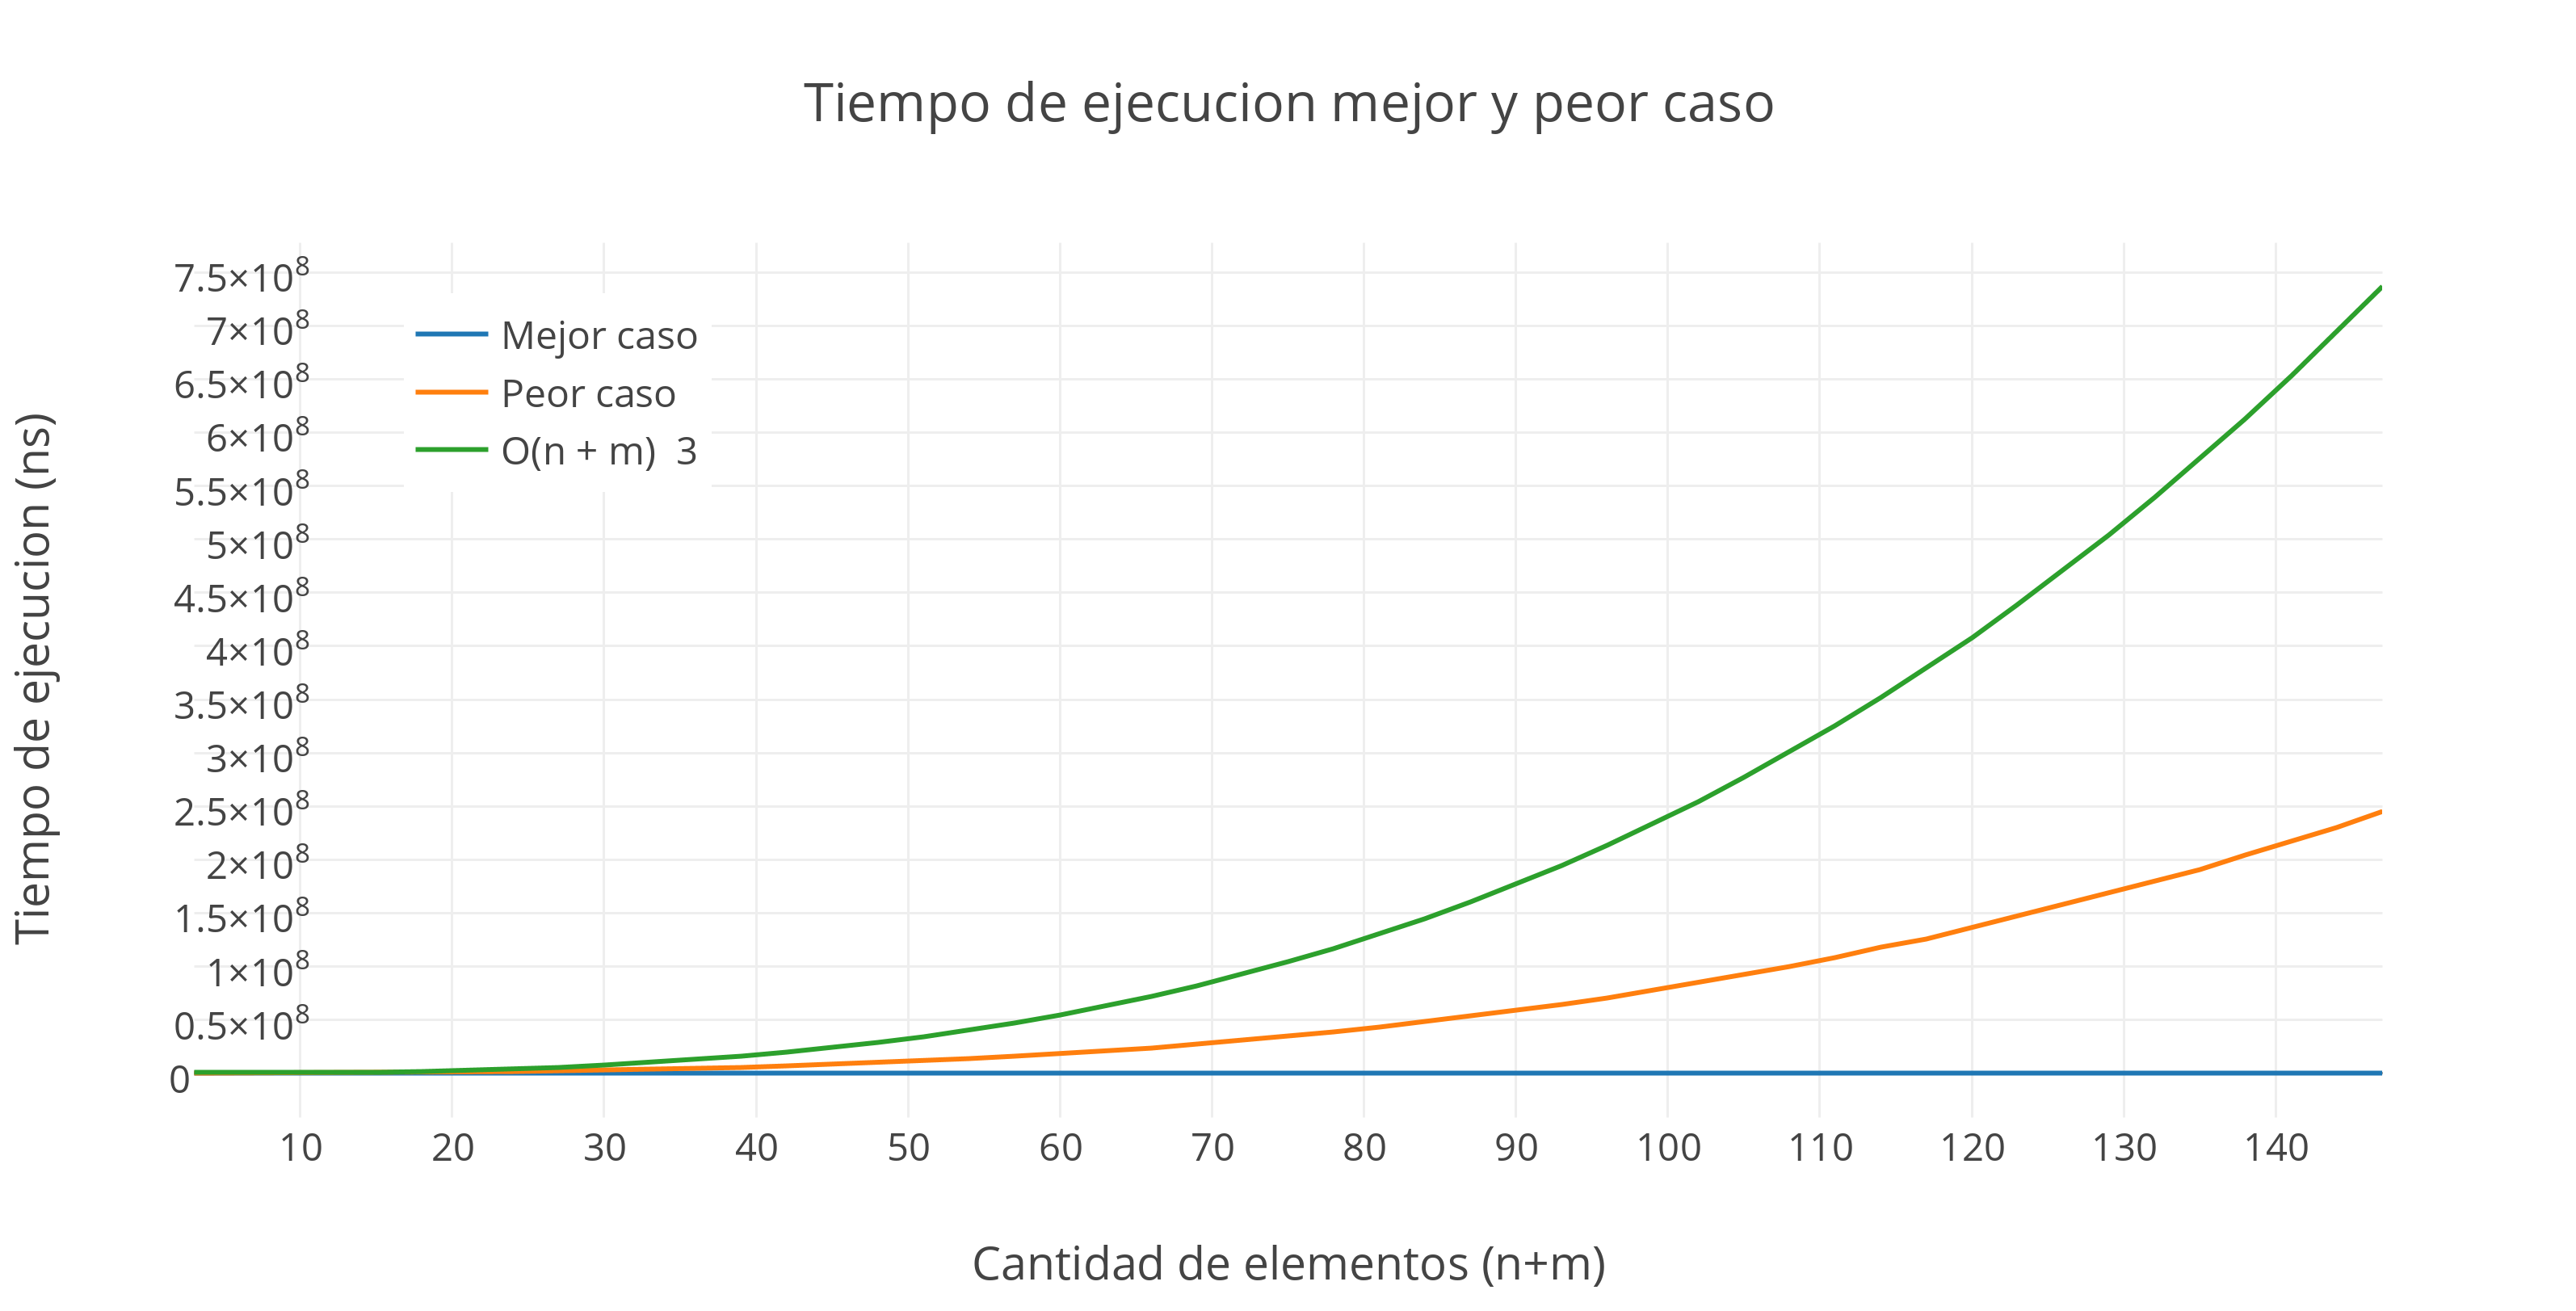
\includegraphics[scale=0.60]{./EJ2/mejorcaso1.png}
\\{\textit{Tiempo de ejecución entre familias}}
  \end{center}
  \vspace*{0.3cm}
  
Es posible observar como las funciones resultantes del mejor y peor caso se encuentran por debajo de la cota de complejidad. Dicha complejidad fue calculada utilizando el m\'etodo de cuadrados m\'inimos generandonos una funcion la cual tomamos como cota dentro de nuestro orden de complejidad $(O(n+m)^3)$.